%%%%%%%%%%%%%%%%%%%%%%%%%%%%%%%%%%%%%%%%%
% Short Sectioned Assignment LaTeX Template Version 1.0 (5/5/12)
% This template has been downloaded from: http://www.LaTeXTemplates.com
% Original author:  Frits Wenneker (http://www.howtotex.com)
% License: CC BY-NC-SA 3.0 (http://creativecommons.org/licenses/by-nc-sa/3.0/)
%%%%%%%%%%%%%%%%%%%%%%%%%%%%%%%%%%%%%%%%%

% \documentclass[paper=a4, fontsize=11pt]{scrartcl} % A4 paper and 11pt font size
\documentclass[11pt, a4paper]{book}
\usepackage[T1]{fontenc} % Use 8-bit encoding that has 256 glyphs
\usepackage[utf8]{inputenc}
\usepackage{fourier} % Use the Adobe Utopia font for the document - comment this line to return to the LaTeX default
\usepackage{listings} % para insertar código con formato similar al editor
%\usepackage[spanish, es-tabla]{babel} % Selecciona el español para palabras introducidas automáticamente, p.ej. "septiembre" en la fecha y especifica que se use la palabra Tabla en vez de Cuadro
\usepackage[hyphens]{url} % ,href} %para incluir URLs e hipervínculos dentro del texto (aunque hay que instalar href)
\usepackage{graphics,graphicx, float} %para incluir imágenes y colocarlas
\usepackage[gen]{eurosym} %para incluir el símbolo del euro
\usepackage{cite} %para incluir citas del archivo <nombre>.bib
\usepackage{enumerate}
\usepackage{enumitem}
\usepackage{hyperref}
\usepackage{graphicx}
\usepackage{tabularx}
\usepackage{booktabs}
\usepackage{multirow}
\usepackage{longtable}
\usepackage{hyperref}
\usepackage{caption}
\usepackage{subcaption}

\usepackage[table,xcdraw]{xcolor}
\hypersetup{
	colorlinks=true,	% false: boxed links; true: colored links
	linkcolor=black,	% color of internal links
	urlcolor=cyan		% color of external links
}
\renewcommand{\familydefault}{\sfdefault}
\usepackage{fancyhdr} % Custom headers and footers
\pagestyle{fancyplain} % Makes all pages in the document conform to the custom headers and footers
\fancyhead[L]{} % Empty left header
\fancyhead[C]{} % Empty center header
\fancyhead[R]{Jesús González Álvarez} % My name
\fancyfoot[L]{} % Empty left footer
\fancyfoot[C]{} % Empty center footer
\fancyfoot[R]{\thepage} % Page numbering for right footer
%\renewcommand{\headrulewidth}{0pt} % Remove header underlines
\renewcommand{\footrulewidth}{0pt} % Remove footer underlines
\setlength{\headheight}{13.6pt} % Customize the height of the header

\usepackage{titlesec, blindtext, color}
\definecolor{gray75}{gray}{0.75}
\newcommand{\hsp}{\hspace{20pt}}
\titleformat{\chapter}[hang]{\Huge\bfseries}{\thechapter\hsp\textcolor{gray75}{|}\hsp}{0pt}{\Huge\bfseries}
\setcounter{secnumdepth}{4}
\usepackage[Lenny]{fncychap}
\DeclareCaptionFont{white}{\color{white}}
\DeclareCaptionFormat{listing}{\colorbox{gray}{\parbox{\textwidth}{#1#2#3}}}
\captionsetup[lstlisting]{format=listing,labelfont=white,textfont=white}
\usepackage{listings}
\renewcommand\lstlistlistingname{List of Code}
\lstset{%
basicstyle=\ttfamily\color{black},
commentstyle = \ttfamily\color{red},
keywordstyle=\ttfamily\color{blue},
stringstyle=\color{orange}}
\lstdefinelanguage{CSharp}
{
 morecomment = [l]{//}, 
 morecomment = [l]{///},
 morecomment = [s]{/*}{*/},
 morestring=[b]", 
 breaklines=true,
 sensitive = true,
 morekeywords = {abstract,  event,  new,  struct,
   as,  explicit,  null,  switch,
   base,  extern,  object,  this,
   bool,  false,  operator,  throw,
   break,  finally,  out,  true,
   byte,  fixed,  override,  try,
   case,  float,  params,  typeof,
   catch,  for,  private,  uint,
   char,  foreach,  protected,  ulong,
   checked,  goto,  public,  unchecked,
   class,  if,  readonly,  unsafe,
   const,  implicit,  ref,  ushort,
   continue,  in,  return,  using,
   decimal,  int,  sbyte,  virtual,
   default,  interface,  sealed,  volatile,
   delegate,  internal,  short,  void,
   do,  is,  sizeof,  while,
   double,  lock,  stackalloc,   
   else,  long,  static,   
   enum,  namespace,  string,
   from, where, select, group, into, orderby, 
	join, let, in, on, equals, by, ascending, descending
   },
}

% Listado definido para JSON
% http://tex.stackexchange.com/questions/83085/how-to-improve-listings-display-of-json-files/83100#83100
\definecolor{delim}{RGB}{20,105,176}
\colorlet{punct}{red!60!black}

\lstdefinelanguage{json}{
	basicstyle=\footnotesize,
	breaklines=true,
	showstringspaces=false,
	literate=
		*{:}{{{\color{punct}{:}}}}{1}
		{,}{{{\color{punct}{,}}}}{1}
	    {\{}{{{\color{delim}{\{}}}}{1}
	    {\}}{{{\color{delim}{\}}}}}{1}
	    {[}{{{\color{delim}{[}}}}{1}
	    {]}{{{\color{delim}{]}}}}{1}
	    {ñ}{{\~{n}}}{1}
}


\begin{document}

	% Plantilla portada UGR
	\begin{titlepage}
\newlength{\centeroffset}
\setlength{\centeroffset}{-0.5\oddsidemargin}
\addtolength{\centeroffset}{0.5\evensidemargin}
\thispagestyle{empty}

\noindent\hspace*{\centeroffset}\begin{minipage}{\textwidth}

\centering

\includegraphics[width=0.9\textwidth]{logos/logo_ugr.jpg}\\[1.4cm]

\textsc{ \Large FINAL DEGREE'S PROJECT\\[0.2cm]}
\textsc{ COMPUTER SCIENCE ENGINEERING}\\[1cm]

{\Huge\bfseries Learn ASL \\}
\noindent\rule[-1ex]{\textwidth}{3pt}\\[3.5ex]
{\large\bfseries Application to learn American Sign Language integrating a deep learning based model. }
\end{minipage}

\vspace{2.5cm}
\noindent\hspace*{\centeroffset}
\begin{minipage}{\textwidth}
\centering

\textbf{Author}\\ {Jesús González Álvarez}\\[2.5ex]
\textbf{Advisor}\\ {Miguel Lastra Leidinger}\\[2cm]

\includegraphics[width=0.3\textwidth]{logos/etsiit_logo.png}\\[0.1cm]
\textsc{Escuela Técnica Superior de Ingenierías Informática y de Telecomunicación}\\
\textsc{---}\\
Granada, Junio de 2022
\end{minipage}
\end{titlepage}


	% Plantilla prefacio UGR
	\thispagestyle{empty}

\begin{center}
{\large\bfseries Learn ASL \\ Application to learn American Sign Language integrating a deep learning based model.}\\
\end{center}
\begin{center}
Jesús González Álvarez\\
\end{center}

%\vspace{0.7cm}

\vspace{0.5cm}
\noindent{\textbf{Keywords}: \textit{open source}
\vspace{0.7cm}

\noindent{\textbf{Abstract}\\
	

\cleardoublepage

\begin{center}
	{\large\bfseries Learn ASL \\ Aplicación para aprender Lenguaje de Signos Americano integrando un modelo de aprendizaje automático.}\\
\end{center}
\begin{center}
	Jesús González Álvarez\\
\end{center}
\vspace{0.5cm}
\noindent{\textbf{Palabras clave}: \textit{software libre}, \textit{floss}
\vspace{0.7cm}

\noindent{\textbf{Resumen}\\

\newpage
\thispagestyle{empty}
\
\vspace{3cm}

\noindent\rule[-1ex]{\textwidth}{2pt}\\[4.5ex]

Yo, \textbf{Jesús González Álvarez}, alumno de la titulación \textbf{Ingeniería Informática} de la \textbf{Universidad de Granada}, autorizo la ubicación de la siguiente copia de mi Trabajo Fin de Grado \textit{Learn ASL} en la biblioteca del centro para que pueda ser consultada por las personas que lo deseen.

\bigskip
El documento en formato {\tt LaTeX} se puede encontrar en el siguiente repositorio de {\tt GitHub}: \url{https://github.com/JesusGonzalezA/LearnASLDoc}.

\vspace{7.5cm}

\noindent Fdo: \textbf{Jesús González Álvarez}

\vspace{2cm}

\begin{flushright}
Granada, a 31 Junio de 2022
\end{flushright}

\newpage
\thispagestyle{empty}
\
\vspace{3cm}

\noindent\rule[-1ex]{\textwidth}{2pt}\\[4.5ex]

D. \textbf{Miguel Lastra Leidinger}, Profesor del Departamento Ingeniería del Software de la Universidad de Granada.


\vspace{0.5cm}

\textbf{Informo:}

\vspace{0.5cm}

Que el presente trabajo, titulado \textit{\textbf{Learn ASL}},
ha sido realizado bajo mi supervisión por \textbf{Jesús González Álvarez}, y autorizo la defensa de dicho trabajo ante el tribunal
que corresponda.

\vspace{0.5cm}

Y para que conste, expiden y firman el presente informe en Granada a Junio de 2022.

\vspace{1cm}

\textbf{El director: }

\vspace{4cm}

\noindent Fdo: \textbf{Miguel Lastra Leidinger}

\vspace{2cm}

\begin{flushright}
Granada, a 31 Junio de 2022
\end{flushright}

\chapter*{Acknowledgments}
\thispagestyle{empty}

\vspace{1cm}

\noindent To my family, who gave me the opportunity to study and values that I really appreciate.

\bigskip
\noindent To all my teachers, from collegue to the university, for their dedication and knowledge.

\bigskip
\noindent To my tutor, Miguel Lastra Leidinger, for believing in me, for his time and special dedication, for his curiosity and intention to help others.








	% Índice de contenidos
	\newpage
	\tableofcontents

	% Índice de imágenes y tablas
	\newpage
	\listoffigures
	
	% Índice de códigos
	\newpage
	\lstlistoflistings

	% Si hay suficientes se incluirá dicho índice
	\listoftables 
	\newpage


	% Introducción 
	This is an open source project under license GNU General Public License \cite{gplv3}. \\

\chapter{Introduction}

Sign or signed languages are complete natural languages that are expressed visually.
They have their own grammar, lexicon and are not universal. \\ 

Sign languages have became the main way of communicating between deaf-and-dumb people. Nevertheless,
it is not common in society to be able to understand them, so the gap between these communities
and the rest of society keeps increasing. \\

As a future Software Engineer, I have a big social responsability, because my developments and ideas
may help minorities and lessen gaps like this one. \\

Solutions such as a videocall application, that subtitles sign languages, could make sign language 
speakers be able to communicate with non-signers.
Although there are a lot of dictionaries and applications to learn sign language, there is an 
absence of applications that verify how you perform signing.
Learning sign language would be easier and more accessible if you would not need someone to do this verification,
and devices are now able to do this.

\section{Preliminar analysis. Viability study.}

In order to create an application to verify a signs or a videocall app, 
translating signs into text would be neccessary. \\

Previous works have their main focus on translating signs into text using special gloves \cite{Gloves}. Although this is effective 
and would solve the problem, not everyone could afford these gloves imposing a barrier to entry. \\

The most accessible hardware for users would be the integrated cameras in their phones and pc's. Therefore,
the main objective of this initial study would be to analyse the efficiency and viability of translating 
a video into text using commodity hardware.

\subsection{Sign language characteristics}
The first thing that comes into mind is to develop a deep learning model able to translate signed sentences into 
text. Firstly, we should know the difficulties that this would take:
\begin{itemize}[noitemsep]
    \item In order to be able to translate a signed sentence into text, the model should understand the context to formulate the sentence correctly.
    \item Some words are signed the same way.
    \item Signs are performed differently if you are left-handed or right-handed.
    \item The dataset should contain videos of people from different ethnicities and sex signing.
\end{itemize}

Just analysing the alphabet would be a much simplier task, as all letters are signed statically (in ASL: American Sign Language), except the 'J' and 'Z'.
Therefore, a classification deep learning model could be developed to validate the images/videos from the user.
Nevertheless, such a system would be of little use and this functaionality has already been developed and implemented by some applications such as \textit{ASL Alphabet by Snapchat} \cite{Snapchat}.

\subsection{Literature review}
This section contains a table \ref{table:introduction_literature_review} with the main sources of information used in this work. \\

\begin{longtable}{|p{3cm}|p{4cm}|p{6cm}|}
    \hline {Type} & {Title} & {Note}      \\
    \hline Video & La INFRAESTRUCTURA detrás de TikTok \cite{TikTok2021} & Infraestructure analysis. How to divide a big service into smaller ones and create an UML diagram from it \\
    \hline Journal & Word-level Deep Sign Language Recognition from Video: A New Large-scale Dataset and Methods Comparison \cite{Li2019} & They introduce a large scale dataset for American Sign Language, consisting of 2000 words performed by more than 100 signers in more than 20.000 videos. They also introduce two models and compare them: holistic visual appearance-based approach, and 2D human pose based approach \\
    \hline Journal & Recognition of user-dependent and independent static hand gestures: Application to sign language \cite{Sadeddine2021} & Sign recognition becomes a very complex tax due to heterogeneous environment. This article studies how to improve accuracy of models using static hand gesture recognition based on a set of image descriptors: Gradient Local Auto-Correlation (GLAC), Gabor Wavelet Transform (GWT), and Fast Discrete Curve Transform (FDCT) \\
    \hline Journal & Optimization of convolutional neural networks architectures using pso for sign language recognition \cite{Fregoso2021} & It presents an approach to design convolutional neural network architectures, using the particle swarm optimization algorithm\\
    \hline Repository & TSPNet: Hierarchical Feature Learning via Temporal Semantic Pyramid for Sign Language Translation \cite{SLTTSPNet} & The repository contains the implementation of a deep learning model to translate from videos to text \\
    \hline Journal & Visual Alignment Constraint for Continuous Sign Language Recognition \cite{Min2021} & Work on how to solve the overfitting problem in recent CTC-based CSLR worksdue to the insufficient training of the feature extractor using a Visual Alignment Constraint (VAC) to enhance the feature extractor with more alignment supervision. It includes a code repository \\
    \hline Journal & ELM based two-handed dynamic Turkish Sign Language (TSL) word recognition \cite{ELM2021} & It studies the recognition of dynamic words in Turkish Sign Language (TSL) with two hands using the Leap Motion Controller (LMC) device \\
    \hline Journal & Applying deep neural networks for the automatic recognition of sign language words: A communication aid to deaf agriculturists \cite{Venugopalan2021} & In order to help deaf agriculturists, they propose a model using a LSTM trained using a small dataset of the most common indian signed-words in this field \\
    \hline Journal & Real-Time Sign Language Detection using Human Pose Estimation \cite{Moryossef2020} & Lightweight real-time sign language detection model for future use in videocall applications \\
    \hline Report  & Sign Language Transformers: Joint End-to-end Sign Language Recognition and Translation \cite{SignLanguageTransformers} & New architecture for continuous sign language recognition \\
    \hline Journal & Sign Language Recognition Using ConvolutionalNeural Networks \cite{Bronstein2015} & Recognition system using the Microsoft Kinect, convolutional neural networks (CNNs) and GPU acceleration \\
    \hline Video   & Real-Time Sign Language Detection for Video Conferencing Applications \cite{RT2021} & System for setting the main signer in a videoconferencing application \\
    \hline Website & American Sign Language Recognition in Python using Deep Learning \cite{ASLRecognitionPython} & Model that uses knowledge transfer to recognise letters in ASL \\
    \hline Website & How to use transfer learning for sign language recognition \cite{Vagdevi2019} & ResNet based model that uses knowledge transfer \\ 
    \hline Website & How to build a convolutional neural network that recognizes sign language gestures \cite{Vagdevi2019i} & Neural network to recognise letters in ASL \\
    \hline Journal & Sign Language Recognition for Computer Vision Enthusiasts \cite{Vaishshells2021} & Two models to recognise letters. A static one and a dynamic one using an american sign language dataset \\
    \hline Journal & ASL Alphabet \cite{Akash2018} & Dataset to sign letters in ASL. It transforms letters 'J' and 'Z' into images because they are signed dynamically (using movement) and requires video recognition. This way, the problem is reduced to an image classification one \\
    \hline Website & Hands-On Guide To Sign Language Classification Using CNN \cite{SignLanguageClassification2020} & Model to classify letters in ASL. It just classify static letters (all except 'J' and 'Z') \\
    \hline Journal & Sign Language Recognition: A Deep Survey \cite{Rastgoo2021} & State of art summary. It contains links to main models, datasets and architectures \\
    \hline Video   & Sign Language Detection using ACTION RECOGNITION with Python | LSTM Deep Learning Model \cite{SignLanguageRecognitionUsingActionRecognition} & Classify some ASL signs from a webcam \\
    \hline Video   & Real Time Sign Language Detection with Tensorflow Object Detection and Python | Deep Learning SSD \cite{SignLanguageRecognitionUsingObjectDetection} & App to recognise 5 static signs. It teaches how to create a dataset, label images and train a model from a dataset \\
    \hline Video   & Building a Real Time Sign Language Detection App with React.JS and Tensorflow.JS | Deep Learning \cite{SignLanguageRecognitionUsingReactjsAndTensorflow} & Shows how to transform a python model to a tensorflow one,upload it to the cloud and download it on the frontend, so that we can use it using a React.js app to validate videos on the client \\
    \hline Journal & Deep Learning Techniques for Spanish Sign Language Interpretation \cite{SpanishDataset2021} & Dataset for Spanish Sign Language recognition. It proposes to use CNNs to classify static letters and RNNs to classify dynamic letters \\
    \hline
    \caption{Literature review}
    \label{table:introduction_literature_review}
\end{longtable}

\subsection{Choosing a solution}
After carefully considering the literature review, my skills and the development time restrictions, I decided to create an application to learn American Sign Language. \\

The reasons that support this decision are:

\begin{itemize}[noitemsep]
    \item Availability of pretrained deep learning models that translate videos of people signing into text.
    \item Attainability of a medium-scale of a real-world dataset (American Sign Language \cite{Li2019}).
    \item Adecuate complexity level. The system is not as simple as the ones that only recognise individual letters and is not limited by a very small dataset.
    \item Competitive differentiation. Other applications are limited to offering users tests to learn sign language \cite{ASLPocket} \cite{Lingvano} or offer dictionary-like search engines to look up a sign \cite{TheASLApp} \cite{LSAmerica}. None offers a solution that integrates artificial intelligence to validate words.
\end{itemize}

\subsubsection{WLASL in depth: A large-scale dataset for Word-Level American Sign Language}
The WLASL was created due to the importance of American Sign Language for the deaf community, and the lack of a large-scale dataset that allows recognition at a word-level and a sentence-level.
It was chosen for this project due to its size and real-world recording conditions.

\paragraph{Characteristics}
The main characteristics of this dataset are:
\begin{itemize}[noitemsep]
    \item It is composed only by \textbf{monocular-RGB} videos: the videos do not rely on special equipment, such as depth cameras, colored gloves...
    \item All signers are in near-frontal views.
    \item The dataset contains 21.083 videos.
    \item Each video contains one sign in ASL.
    \item The videos are performed by 119 signers.
    \item Each sign is performed by at least 3 different signers.
    \item The average is 2.41 seconds (from 0.36 to 8.12 seconds).
\end{itemize}

\paragraph{Dataset structure}
The dataset is divided into four parts as shown on table \ref{table:introduction_dataset_subdivisions}.
\begin{table}[h]
    \centering
    \resizebox{\textwidth}{!}{
    \begin{tabular}{|c|c|c|c|c|c|}
        \cline{1-6}  Datasets   & Gloss &  Videos &  Mean  & Signers   & Year       \\
        \hline       WLASL100   &   100 &   2,038 &  20.4  &      97   & 2019       \\
        \hline       WLASL300   &   300 &   5,117 &  17.1  &     109   & 2019       \\
        \hline      WLASL1000   &  1000 &  13,168 &  13.2  &     116   & 2019       \\
        \hline      WLASL2000   &  2000 &  21,083 &  10.5  &     119   & 2019       \\
        \hline
    \end{tabular}
    }
\caption{WLASL dataset structure}
\label{table:introduction_dataset_subdivisions}
\end{table}

\paragraph{Models proposed} The paper associated to the WLASL dataset proposes two models:
\begin{itemize}[noitemsep]
    \item I3D: it follows a I3D network architecture \ref{fig:introduction_i3d}. It is trained using ImageNet \cite{ImageNet} 
    and finetuned using Kinetics-400 \cite{Kinetics400}. Since the class number varies depending on
    the dataset, the last classification layer is changed according to it. \\
    \begin{figure}[H]
        \centering
            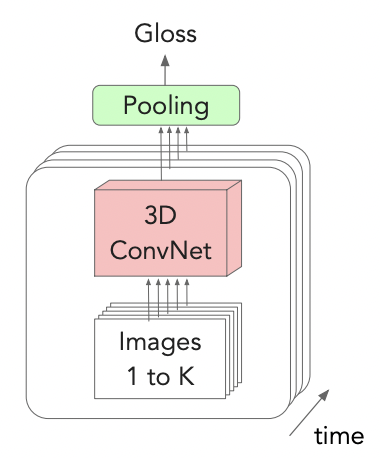
\includegraphics[width=0.4\textwidth]{assets/i3d.png}
        \caption{I3D architecture}
        \label{fig:introduction_i3d}
    \end{figure}
    \item Pose TGCN: pose based temporal graph neural network \ref{fig:introduction_tgcn}. Usually, motion is modelled using 2D joint angles.
    They encode the motion using a holistic representation of the trajectories of body keypoints. They represent
    the human body as a fully-connected graph to learn the dependencies between joints in the trajectories.
    \begin{figure}[H]
        \centering
            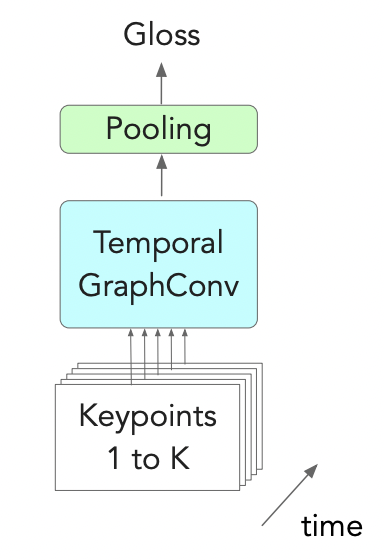
\includegraphics[width=0.4\textwidth]{assets/tgcn.png}
        \caption{TGCN architecture}
        \label{fig:introduction_tgcn}
    \end{figure}
\end{itemize}

\subparagraph{Data pre-processing} They following transformations are applied:
\begin{itemize}[noitemsep]
    \item Resize the original resolution so that the bounding-box size of the signer is 256x256 pixels.
    \item Crop a 224x224 patch from the input frame.
    \item Apply a horizontal flipping with a prob of 0.5.
\end{itemize}

\subparagraph{Implementation details and accuracy evaluation} The models are all implemented using Pytorch and the top 10 accuracy values are shown on table \ref{fig:introduction_model_accuracy_comparison}. \\
\begin{figure}[H]
    \centering
        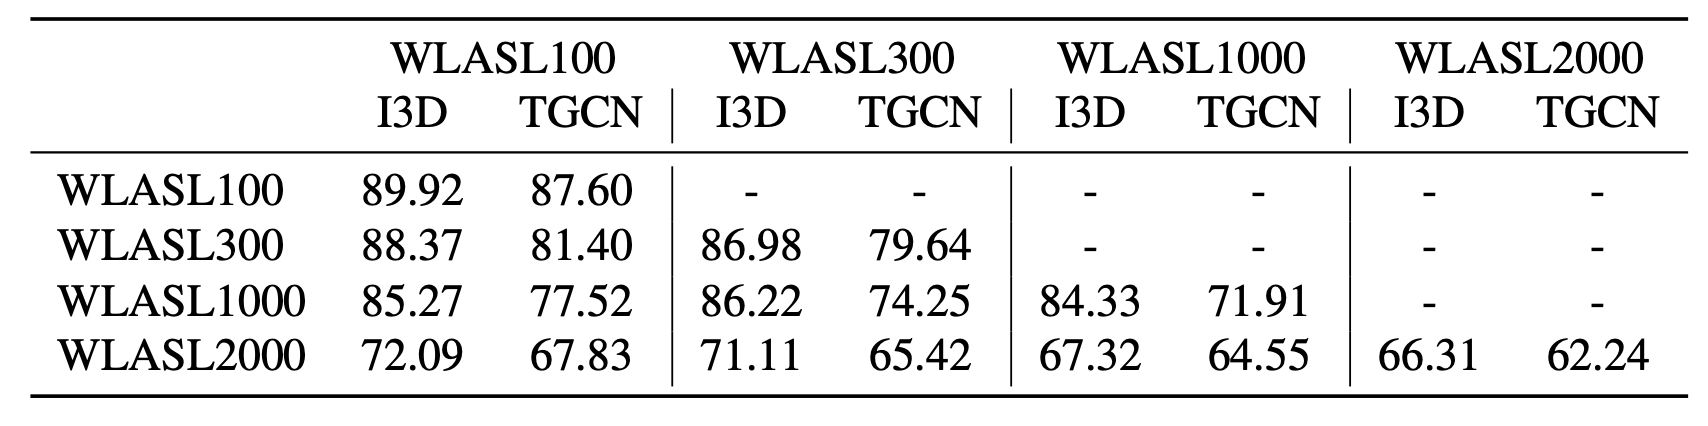
\includegraphics[width=1.0\textwidth]{assets/models_accuracy.png}
    \caption{Models' accuracy comparison}
    \label{fig:introduction_model_accuracy_comparison}
\end{figure}

I decided to use the I3D model due to its better performance.


	% Descripción del problema y hasta donde se llega
	\chapter{Problem description}

There is a big gap between deaf and dumb communities and the rest of society. Sign languages are vital for deaf and dumb people to communicate, and this gap is even bigger because most of people does not know how to sign. \\

In addition, old studies use expensive hardware, which make the learning process of sign language even less accesible. \\ 

In order to lessen this gap, an application is planned to be developed, using just integrated hardware of user's devices. Therefore, people will have a new resource to learn how to sign and validate if they are performing correctly.

\section{Description of the application}
The application, \textbf{Learn ASL}, is planned to be a web application, as it should be accesible to every device and every operative system.
The main objective of the application is to allow users to learn words in sign language and verify if they are signing correctly. \\

This way, the user would be able to do tests. In these tests the user would be asked:
\begin{itemize}
    \item \textbf{A word:} 
        \begin{itemize}
            \item The user would select the video that matches.
            \item The user would sign the word and the application would verify if the signed word in the video matches.
        \end{itemize}
    \item \textbf{A video:} The user would select the word that matches.
\end{itemize}

\subsection{Requisites of the application}
\begin{itemize}
    \item Internet connection.
    \item Integrated camera or external camera.
    \item An email account is required.
\end{itemize}

\section{Objectives}

\section{User stories}


	
	% Análisis del problema
	% 1. Análisis de requisitos
	% 2. Análisis de las soluciones
	% 3. Solucion propuesta
	% 4. Análisis de seguridad
	\chapter{Analysis}

\section{Objectives}
The main objectives of the app to be developped, thinking of them as high-level requisites, are the following ones: 

\begin{enumerate}[label=\textbf{Obj\_\arabic*:}, align=left, leftmargin=*]
    \item The system will manage and keep all the information related to users, such as their credentials, done tests and stats.
    \item The system will update the users' stats automatically after every done test. 
    \item The system will allow the users to manage their account.
    \item The system will allow the users to read their stats and done tests.
    \item The system will manage the tests, being capable of creating them every time a user request to start one.
    \item The system will store the videos of the users signing and will manage its visibility (to hide the videos to other users so that privacy is achieved).
\end{enumerate}

\section{Requirements}
\subsection{Functional requirements}
\begin{enumerate}[label=\textbf{RF\_\arabic*}, align=left, leftmargin=*]
    \item Users management:
        \begin{enumerate}[label=\textbf{\theenumi.\arabic*}, align=left, leftmargin=*]
            \item The system will allow a non registered user be signed up in the the system.
            \item The system will store all the information relative to the user in order to be able to identify them before entering the app.
            \item The system will allow a registered user and identified to delete their account and information.
        \end{enumerate}
    \item Tests management: 
        \begin{enumerate}[label=\textbf{\theenumi.\arabic*}, align=left, leftmargin=*]
            \item The system will be able to generate all different types of tests:
                \begin{itemize}
                    \item \textit{Mimic tests}
                    \item \textit{QA tests}
                    \item \textit{Option tests}
                        \begin{itemize}
                            \item \textit{Word to video test}
                            \item \textit{Video to word test}
                        \end{itemize}
                    \item \textit{Error test} variant from all the tests above
                \end{itemize}
            \item The system will be able to generate tests depending on the difficulty level. The difficulty will be \textit{EASY}, \textit{MEDIUM} and \textit{HARD}, depending on the selected dataset, \textit{WLASL300},  \textit{WLASL1000},  \textit{WLASL2000} respectively.
            \item The system will allow the user to review an already done test and its results.
            \item The system will protect the review of tests, so that only the user who did the test is able to review it.
            \item The system will allow the user to delete all the done tests.
        \end{enumerate}
    \item Analytics management: The system will create stats from the tests done by the user until the moment the stats are required.
        \begin{enumerate}[label=\textbf{\theenumi.\arabic*}, align=left, leftmargin=*]
            \item The system will create stats and display diagrams from the following topics:
                \begin{enumerate}
                    \item Success percent.
                    \item Percent of learnt words.
                    \item Days the user has started a test in the app.
                    \item New learnt words.
                \end{enumerate}
            \item The system will allow the user to filter the stats by difficulty and date.
        \end{enumerate}
\end{enumerate}

\subsection{Non-Functional requirements}
\begin{enumerate}[label=\textbf{RNF\_\arabic*}, align=left, leftmargin=*]
    \item \textbf{Open source:} The application should be open source, due to its social interest.
    \item \textbf{Accessibility: } The application should be accesible. Therefore, a well-tested UI library should be used and there will be no action that depends on sounds.
    \item \textbf{Usability:} The application should be responsive.
    \item \textbf{Maintenability:} The application core should be under a clean architecture, so that the maintenance of the application is guaranteed to be an easier task.
    \item \textbf{Testability:} The main core of the application should be tested using unit tests.
    \item \textbf{Privacy:} The application will require authorization and authentication in order to let a user interact with the system. The user will only be granted to access their own resources.
\end{enumerate}

\section{User's stories}
In order to write the stories and follow their development, I created a project in GitHub. You can access it here \url{https://github.com/JesusGonzalezA/LearnASL/projects/3}. \\

I divided the user stories in three main categories, according to the Functional Requirements:
\begin{enumerate}[label=\textbf{US\_\arabic*}, align=left, leftmargin=*]
    \item \textbf{User management} 
        \begin{enumerate}[label=\textbf{\theenumi.\arabic*}, align=left, leftmargin=*]
            \item As a non signer, I want to register in the app to learn American Sign Language.
            \item As an user, I want to login in the app.
            \item As an user, I want to change my password.
            \item As an user, I want to delete my account.
            \item As an user who does not remember their password, I want to be able to recover my account.
            \item As an already registered user, I want to update my email.
        \end{enumerate}
    \item \textbf{Test management} 
        \begin{enumerate}[label=\textbf{\theenumi.\arabic*}, align=left, leftmargin=*]
            \item As an user, I want to start a new test.
            \item As an user, I want to select the difficulty of a test.
            \item As an user, I want to customize the number of questions of a test.
            \item As an user, I want to know my result in the test.
            \item As an user, I want to see in which question I am on.
            \item As an user, I want to review a test done in the past.
            \item As a user, I want to see a list with all the tests I've made.
        \end{enumerate}
    \item \textbf{Stats management}
        \begin{enumerate}[label=\textbf{\theenumi.\arabic*}, align=left, leftmargin=*]
            \item As an user, I want to select the interval of time of my stats.
            \item As an user, I want to review my stats.
            \item As an user, I want to delete my history of tests.
        \end{enumerate}
\end{enumerate}

\subsection{Milestones}
Each milestone represents a group of user stories that can be grouped in order to present a value increase. The objective of define the milestones is that, due to the fact that I am not going to work full-time on the project, I cannot organize review meetings and fixed deadlines. This way, I can get feedback from every milestone's completion until the final product is achieved. \\

\begin{enumerate}[label=\textbf{MIL\_\arabic*}, align=left, leftmargin=*]
    \item Project set up
        \begin{enumerate}[label=\textbf{\theenumi.\arabic*}, align=left, leftmargin=*]
            \item Both backend and frontend projects are initialized.
            \item The test and production environments are set up.
            \item The project is containerized.
            \item The Github actions are prepared.
        \end{enumerate}
    \item Authentication
        \begin{enumerate}[label=\textbf{\theenumi.\arabic*}, align=left, leftmargin=*]
            \item A user can register/login/log out/sign off/change password/change email. Refers to \textit{US\_1}.
            \item There are private/public routes and screens.
        \end{enumerate}
    \item The app is designed
        \begin{enumerate}[label=\textbf{\theenumi.\arabic*}, align=left, leftmargin=*]
            \item A good Readme is created.
            \item Figma \cite{Figma} Low-Fidelity design.
            \item Figma \cite{Figma} High-Fidelity design.
        \end{enumerate}
    \item A web version of the app is avalaible
        \begin{enumerate}[label=\textbf{\theenumi.\arabic*}, align=left, leftmargin=*]
            \item React version of the application with faked data.
        \end{enumerate}
    \item The app can create tests
        \begin{enumerate}[label=\textbf{\theenumi.\arabic*}, align=left, leftmargin=*]
            \item The app can create tests. Refers to \textit{US\_2.1}.
            \item The user can upload a video. Refers to \textit{US\_2}.
            \item The user can start a new test. Refers to \textit{US\_2.1}.
        \end{enumerate}
    \item The app saves info
        \begin{enumerate}[label=\textbf{\theenumi.\arabic*}, align=left, leftmargin=*]
            \item A user can crud information about themselves. Refers to \textit{US\_1, US\_2, US\_3}.
            \item A user can watch past tests. Refers to \textit{US\_2.4, US\_2.6}.
            \item A user can delete old tests. Refers to \textit{US\_3.3}.
        \end{enumerate}
    \item Graphical stats
        \begin{enumerate}[label=\textbf{\theenumi.\arabic*}, align=left, leftmargin=*]
            \item The user can see the data in a graphical way. Refers to \textit{US\_3.1, US\_3.2}.
        \end{enumerate}
    \item The app validates the videos
        \begin{enumerate}[label=\textbf{\theenumi.\arabic*}, align=left, leftmargin=*]
            \item The app validates the videos. Refers to \textit{US\_2}.
            \item The user is able to see the result of the test.  Refers to \textit{US\_2.4, US\_2.6, US\_2.7}.
        \end{enumerate}
    \item Migrating to React Native or PWA
    \item Using custom Deep Learning model or improving the existing one
\end{enumerate}
  
\section{Tool's selection}
The main reason why I chosed these technologies is because they would allow me to develop the application and I've already some experience with them. \\ 

This way, I could minimize the risk of the development process and get the first MVP as soon as possible. \\

In addition, all technologies are standards in industry and learning more about them will allow me to fit better in the market. \\ 

Although I have more experience using other technologies, as they are requirements in the degree, I beleive this stack fits better my neccessities and are better adapted to this type of development.

\begin{table}[h]
    \centering
    \resizebox{\textwidth}{!}{
    \begin{tabular}{|p{3cm}|p{2cm}|p{4cm}|p{2cm}|p{4cm}|}
        \cline{1-5} Type & Tool & Description & Experience & Reason to choose it       \\
        \hline \multirow{5}{*}{Version control}   & Git     & Program to manage the different versions of a directory   & Y & Standard and experience \\
        \cline{2-5}                               & GitHub  & To host my git repository                                 & Y & Standard, experience and ability to use GitHub's projects and CI tools \\
        \hline \multirow{5}{*}{Backend}   & ASP.NET core   & C-Sharp framework to create REST API & Y & Standard and experience \\
        \cline{2-5}                       & Flask          & Python framework to create REST API  & N & Standard and ease to integrate with PyTorch \\
        \hline \multirow{5}{*}{Frontend}  & React.js    & Javascript library used to create SPA applications & Y & Standard and experience \\
        \cline{2-5}                       & Typescript  & Programming language                               & Y & Standard, experience, typed language \\
        \hline \multirow{5}{*}{Testing}  & xUnit    & Library to test ASP.NET applications & N & I had a project from Vilnius University where I had to use it and it was a recommendation of my teacher \\
        \cline{2-5}                      & Postman  & Application to do API calls, load tests, simple unit tests and integration tests to REST APIs & Y & There is a new feature that I want to try \\
        \cline{2-5}                      & Chai.js  & Library to do javascript tests. & N & Legacy by Postman \\
        \hline \multirow{5}{*}{Documentation}  & Draw.io    & Web application to design graphs and diagrams & Y & It does not need any license and it is intuitive \\
        \cline{2-5}                      & Swagger  & library to document the endpoints of the application & Y & I prefer it rather than using other's such as Postman due to its integration in the language \\
        \cline{2-5}                      & GitHub projects  & In order to do my planification, set up my sprints and follow the development process & Y & I'm already using GitHub \\
        \hline \multirow{5}{*}{Database}  & Microsoft SQL Server &  DBMS from Microsoft & Y & Experience and ease to integrate with ASP.NET Core \\
        \cline{2-5}                      & Entity framework  & ORM to work with databases for .NET applications & Y & Experience, standard, documentation and good integration \\
        \cline{2-5}                      & Azure data studio  & Program to connect to an existing DB, execute SQL statements, edit tuples... & Y & I prefer to work from a GUI \\
        \hline \multirow{5}{*}{Styling}  & Figma & Application to design mockups and high fidelity projects & Y & Standard, experience and easy to use \\
        \cline{2-5}                      & Material.ui & components library from Google & N & They take accessibility into account, it is stable and good looking \\
        \hline \multirow{5}{*}{CI}  & Microsoft SQL Server &  DBMS from Microsoft & Y & Experience and ease to integrate with ASP.NET Core \\
        \hline
    \end{tabular}
    }
\caption{Tool's selection analysis}
\label{table:analysis_tools_selection}
\end{table}


	\chapter{Planification}

\section{Methodology}
Usually in the degree, we use a waterfall model to develop. For small projects and use cases this methodology \\
works fine, but in bigger projects it carries a lot of issues. \\

In addition, it does not make sense to design all the system in earlier iterations, due to the fact that I \\
don't really have much experience using these technologies, so my diagrams will change a lot in the future. \\
This way, I should mantein both codebase and designs, and designs will be changed a lot and won't be very useful. \\

In conclusion, although waterfall model is the most used in the degree, I opted to use an agile methodology and reiterate \\
the design process, so I'm flexible and I only design what it is really neccessary to me in order to develop the app and mantein the codebase later on. \\

At first, I used a process similar to waterfall model. I captured all the requirements, I design in a very basic way the app and I started developing the architecture. \\
Later on, I would change the design, and the architecture itself, but that will come in the implementation chapter later. \\

\begin{figure}[H]
    \begin{center}
        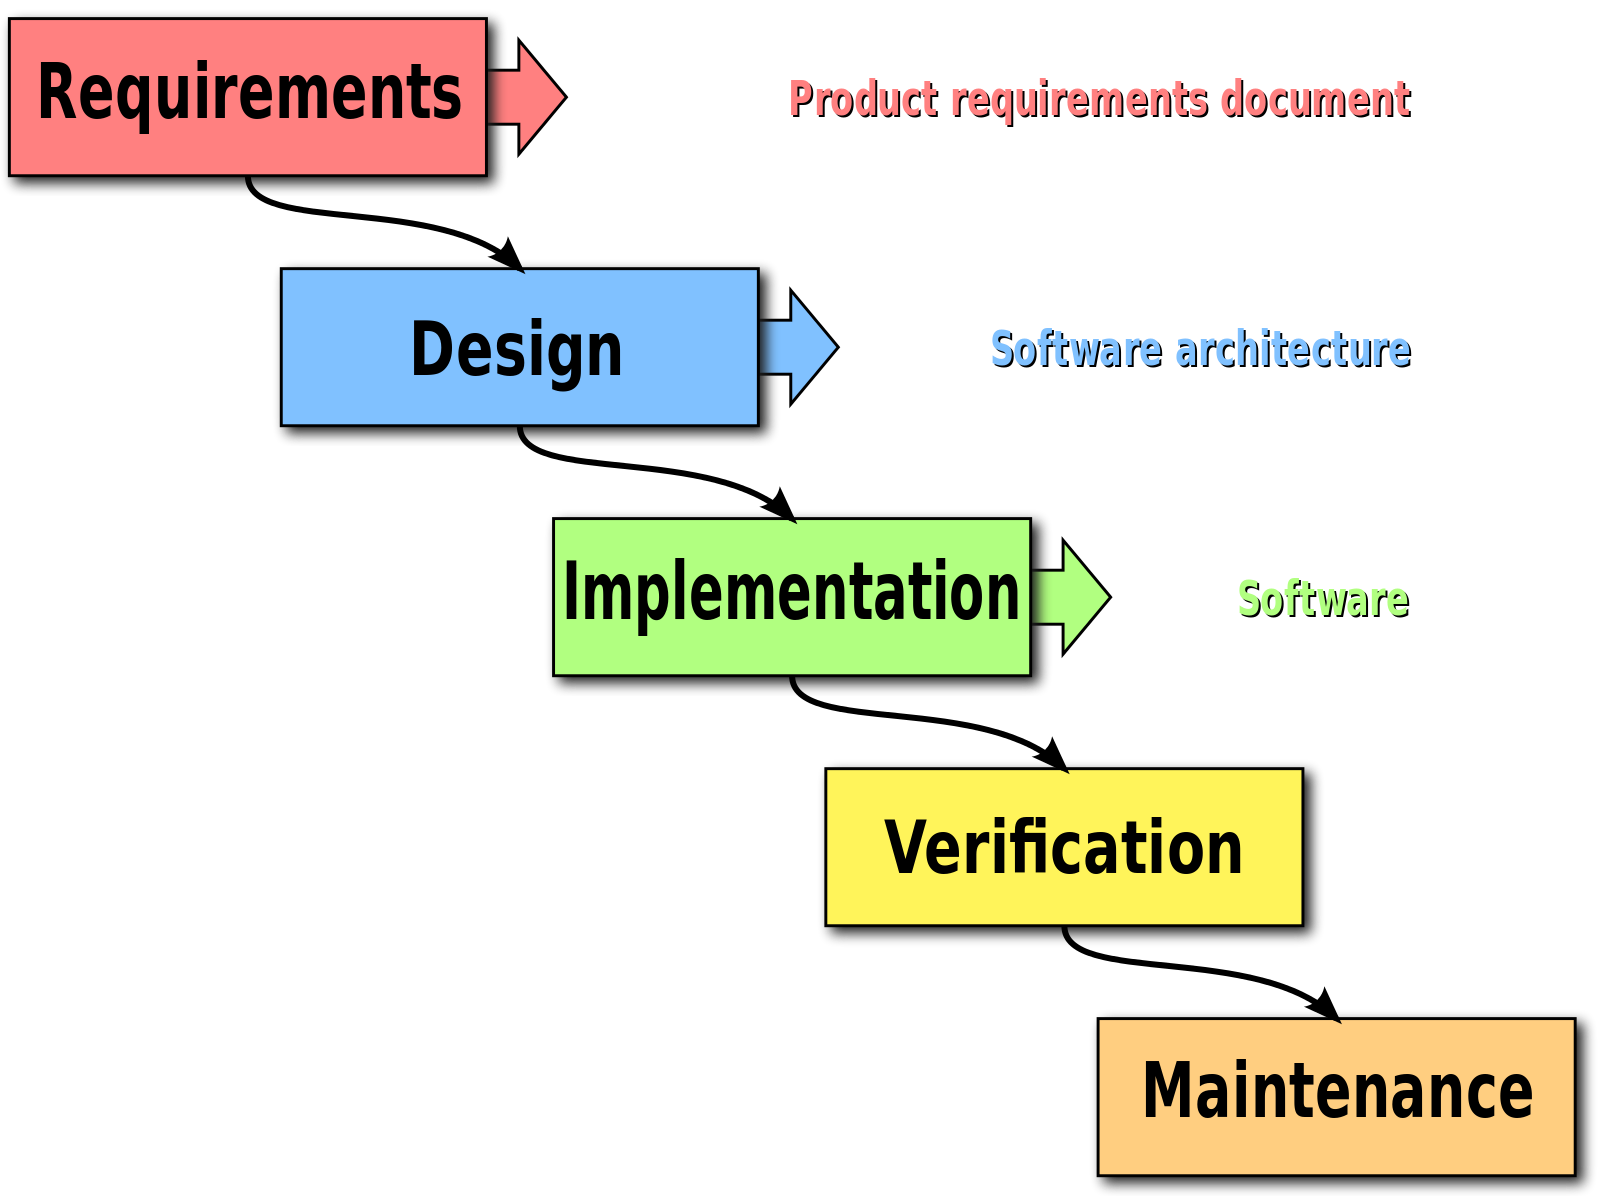
\includegraphics[width=0.4\textwidth]{assets/waterfall_model.png}
        \caption{Waterfall Model. \cite{Waterfall}}
        \label{fig:planification_waterfall_model}
    \end{center}
\end{figure}

In the Scrum model we iterate every fixed amount of time and start a new waterfall model. \\
We critize what could be changed to implement and develop in a better way and we reorder the tasks. \\
Me, instead of having fixed sprints, I used this methodology but the amount of time of every sprint was flexible. It was the neccessary time in order to achieve a new product with a value increase. \\

\begin{figure}[H]
    \begin{center}
        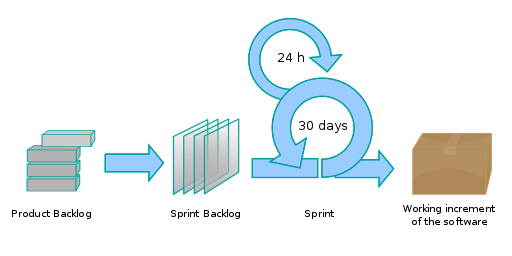
\includegraphics[width=0.4\textwidth]{assets/scrum.png}
        \caption{Scrum Model. \cite{Scrum}}
        \label{fig:planification_scrum_model}
    \end{center}
\end{figure}

Firstly, I recognised all the tasks that I should complete in order to develop the application and the thesis itself. I divided into groups:
\begin{itemize}[noitemsep]
    \item Literature review
    \item Backend
    \item Frontend
    \item Deep Learning service
    \item Documentation
    \item Design
\end{itemize}

Then I grouped the tasks in order to deliver a new product that represents a value increase. \\
This new product should be validated, so a meeting with the tutor was appointed. \\
Then, the rest of the active tasks were given a priority and grouped to form the new iteration backlog. \\
There were a lot of replanification, this was due to:
\begin{itemize}[noitemsep]
    \item Unexperience. I was not able to correctly planificate the tasks, although I splitted them into smaller ones. I was sometimes stuck in some of them and others required less work load than expected.
    \item Flexible project schedule. I was aware of my lack of experience and that I was going to fail in this task, so I tried to bring my deadline earlier so that I had more time.
    \item Subjects: In my Erasmus University we had some subjects in which we studied in depth C-Sharp, ASP.NET core and React Native. I was not aware of it, so I replanificated my tasks related to this thesis so that I could work on them after studying the technology in the subject to gain time.
    \item Uncertainties: Travels, plans, exams, deadline from the university, technical interviews...
\end{itemize}

\section{Temporarization}
In order to create my project schedule, I used Notion \cite{Notion}. You can check my planifications \href{https://cyclic-chiller-238.notion.site/LearnASL-60bb8f91ed8f4ccfa90f98ee2306403d}{here}. \\

\subsection{Theorical project schedule}
\begin{table}[H]
    \centering
    \resizebox{\textwidth}{!}{
    \begin{tabular}{|l|l|l|l|}
        \cline{1-4}      Name                                &    Milestone                                                              &    Due                                           &       State   \\
        \hline           Project set up                      &    \href{https://github.com/JesusGonzalezA/LearnASL/milestone/1}{Link}      &    November 12, 2021                             &       No      \\
        \hline           Graphical Stats                     &    \href{https://github.com/JesusGonzalezA/LearnASL/milestone/8}{Link}      &    February 4, 2022    →   February 11, 2022     &       No      \\
        \hline           The app saves info                  &    \href{https://github.com/JesusGonzalezA/LearnASL/milestone/7}{Link}      &    January 7, 2022     →   January 14, 2022      &       No      \\
        \hline           The app can create tests            &    \href{https://github.com/JesusGonzalezA/LearnASL/milestone/4}{Link}      &    December 31, 2021   →   January 7, 2022       &       No      \\
        \hline           Frontend avalaible                  &    \href{https://github.com/JesusGonzalezA/LearnASL/milestone/3}{Link}      &    December 10, 2021   →   December 31, 2021     &       No      \\
        \hline           The app is designed                 &    \href{https://github.com/JesusGonzalezA/LearnASL/milestone/2}{Link}      &    December 3, 2021    →   December 17, 2021     &       No      \\
        \hline           The user is authenticated           &    \href{https://github.com/JesusGonzalezA/LearnASL/milestone/6}{Link}      &    November 12, 2021   →   December 3, 2021      &       No      \\
        \hline           The app validates the videos        &    \href{https://github.com/JesusGonzalezA/LearnASL/milestone/5}{Link}      &    February 11, 2022   →   February 25, 2022     &       No      \\
        \hline           Using own ML model                  &    \href{https://github.com/JesusGonzalezA/LearnASL/milestone/10}{Link}     &                                                  &       No      \\
        \hline           Migrating to React Native or PWA    &    \href{https://github.com/JesusGonzalezA/LearnASL/milestone/9}{Link}      &                                                  &       No      \\
        \hline
    \end{tabular}
    }
\caption{Theorical project schedule}
\label{table:planification_theorical_project_schedule}
\end{table}

\subsection{Real project schedule}
I changed the order of the milestones. I decided to develop the backend of the application first, instead of the frontend or implementing them in the same time. \\

This decision was made because focusing on the same technology would allow me to go faster because I don't have to change the context and I was learning ASP.NET core in my  \\
university, so I could ask my teachers for help and it also helped me to study. \\
\begin{table}[H]
    \centering
    \resizebox{\textwidth}{!}{
    \begin{tabular}{|l|l|l|l|l|}
        \cline{1-5}      Name                                           &    Milestone                                              &       Due                                     & State & Tag       \\
        \hline           Project set up                                 & \href{https://github.com/JesusGonzalezA/LearnASL/milestone/1}{Link}    &       November 12, 2021                       & Yes   & Backend, Frontend \\
        \hline           Implement authorization and authentication     & \href{https://github.com/JesusGonzalezA/LearnASL/milestone/6}{Link}    &       November 12, 2021 → December 3, 2021    & Yes   & Backend   \\
        \hline           The app can create tests: just word to video   &                                                        &       December 3, 2021  → January 7, 2022      & No    & Backend   \\
        \hline           The app can create the rest of tests           & \href{https://github.com/JesusGonzalezA/LearnASL/milestone/4}{Link}    &       January 7, 2022   → January 21, 2022      & No    & Backend   \\
        \hline           The app create stats                           & \href{https://github.com/JesusGonzalezA/LearnASL/milestone/8}{Link}    &       January 21, 2022  → January 28, 2022     & No    & Backend   \\
        \hline           The app is designed                            & \href{https://github.com/JesusGonzalezA/LearnASL/milestone/2}{Link}    &       January 28, 2022  → February 4, 2022     & No    & Frontend  \\
        \hline           Frontend avalaible                             & \href{https://github.com/JesusGonzalezA/LearnASL/milestone/3}{Link}    &       February 4, 2022  → March 4, 2022        & No    & Frontend  \\
        \hline           Connect frontend and backend                   &                                                         &       March 4, 2022     → March 11, 2022          & No    & Frontend  \\
        \hline           The app validates the videos                   & \href{https://github.com/JesusGonzalezA/LearnASL/milestone/5}{Link}    &       March 11, 2022    → April 1, 2022          & No    & Backend   \\
        \hline           Using own ML model                             & \href{https://github.com/JesusGonzalezA/LearnASL/milestone/10}{Link}   &                                               & No    & Backend   \\
        \hline           Migrating to React Native or PWA               & \href{https://github.com/JesusGonzalezA/LearnASL/milestone/9}{Link}    &                                               & No    & Frontend  \\
        \hline
    \end{tabular}
    }
\caption{Modification v1}
\label{table:planification_real_v1}
\end{table}

The next modification was made because I did not take into account the task of documenting what I was implementing, and I had to divide the task in \textit{Frontend} as well. \\

Also, I underestimated how much time doing unit tests was going to take me. This was because in the subject we were going to learn them in depth, but we finally did not \\
focused on one single framework, so I had to learnt it by myself. \\
\begin{table}[H]
    \centering
    \resizebox{\textwidth}{!}{
    \begin{tabular}{|l|l|l|l|l|}
        \cline{1-5}      Name                                           &    Milestone                                              &       Due   & State & Tag  \\
        \hline Project set up & \href{https://github.com/JesusGonzalezA/LearnASL/milestone/1}{Link} & November 12, 2021 & Yes & Backend, Frontend    \\
        \hline Implement authorization and authentication & \href{https://github.com/JesusGonzalezA/LearnASL/milestone/6}{Link} & November 12, 2021 → December 3, 2021 & Yes & Backend   \\
        \hline The app can create tests & \href{https://github.com/JesusGonzalezA/LearnASL/milestone/4}{Link} & December 3, 2021 → January 7, 2022 & Yes & Backend   \\
        \hline The app create stats & \href{https://github.com/JesusGonzalezA/LearnASL/milestone/8}{Link} & January 1, 202 → January 7, 202 & Yes & Backend  \\
        \hline Documentate &  & January 6, 2022 → January 11, 2022 & Yes & Backend  \\
        \hline Integration tests api &  & January 12, 2022 → January 26, 2022 & No & Backend    \\
        \hline The app is designed & \href{https://github.com/JesusGonzalezA/LearnASL/milestone/2}{Link} & January 26, 2022 → February 4, 2022 & No & Frontend   \\
        \hline User management &  & February 4, 2022 → February 11, 2022 & No & Frontend    \\
        \hline Test management &  & February 11, 2022 → February 21, 2022 & No & Frontend   \\
        \hline Stats management &  & February 21, 2022 → February 28, 2022 & No & Frontend  \\
        \hline The app validates the videos & \href{https://github.com/JesusGonzalezA/LearnASL/milestone/5}{Link} & February 28, 2022 → March 20, 2022 & No & Backend    \\
        \hline Using own ML model & \href{https://github.com/JesusGonzalezA/LearnASL/milestone/10}{Link} &  & No & Backend   \\
        \hline Migrating to React Native or PWA & \href{https://github.com/JesusGonzalezA/LearnASL/milestone/9}{Link} &  & No & Frontend \\
        \hline Integrate with google analytics &  &  & No & Frontend \\
        \hline
    \end{tabular}
    }
\caption{Modification v2}
\label{table:planification_real_v2}
\end{table}

This modification was made due to a good new. Doing the unit tests, after learning the framework, did not take me that amount of time. \\

Therefore, I modify the planification to rest some days and dedicate myself to design the app more days. \\
\begin{table}[H]
    \centering
    \resizebox{\textwidth}{!}{
    \begin{tabular}{|l|l|l|l|l|}
        \cline{1-5}      Name                                           &    Milestone                                              &       Due   & State & Tag  \\
        \hline Project set up & \href{https://github.com/JesusGonzalezA/LearnASL/milestone/1}{Link} & November 12 , 2021 & Yes & Backend, Frontend \\
        \hline Implement authorization and authentication & \href{https://github.com/JesusGonzalezA/LearnASL/milestone/6}{Link} & November 12 , 2021 → December 3 , 2021 & Yes & Backend \\
        \hline The app can create tests & \href{https://github.com/JesusGonzalezA/LearnASL/milestone/4}{Link} & December 3 , 2021 → January 7 , 2022 & Yes & Backend \\
        \hline The app create stats & \href{https://github.com/JesusGonzalezA/LearnASL/milestone/8}{Link} & January 1 , 202 → January 7 , 202 & Yes & Backend \\
        \hline Documentate &  & January 6 , 2022 → January 11 , 2022 & Yes & Backend \\
        \hline Integration tests api &  & January 12 , 2022 → January 15 , 2022 & Yes & Backend \\
        \hline The app is designed & \href{https://github.com/JesusGonzalezA/LearnASL/milestone/2}{Link} & January 18 , 2022 → February 4 , 2022 & No & Frontend \\
        \hline User management &  & February 4 , 2022 → February 11 , 2022 & No & Frontend \\
        \hline Test management &  & February 11 , 2022 → February 21 , 2022 & No & Frontend \\
        \hline Stats management &  & February 21 , 2022 → February 28 , 2022 & No & Frontend \\
        \hline The app validates the videos & \href{https://github.com/JesusGonzalezA/LearnASL/milestone/5}{Link} & February 28 , 2022 → March 20 , 2022 & No & Backend \\
        \hline Using own ML model & \href{https://github.com/JesusGonzalezA/LearnASL/milestone/10}{Link} &  & No & Backend \\
        \hline Migrating to React Native or PWA & \href{https://github.com/JesusGonzalezA/LearnASL/milestone/9}{Link} &  & No & Frontend  \\
        \hline Integrate with google analytics &  &  & No & Frontend \\
        \hline
    \end{tabular}
    }
\caption{Modification v3}
\label{table:planification_real_v3}
\end{table}

The next modification was made because the frontend task took me more than expected. I was working but I had a lot of uncertainties. \\

Because of this, I gave priority to integrating the deep learning model. This was the most risky task, due to my lask of knowledge on the field. \\

In addition, I added some tasks, such as creating this document itself or improving the ai service. \\
\begin{table}[H]
    \centering
    \resizebox{\textwidth}{!}{
    \begin{tabular}{|l|l|l|l|l|}
        \cline{1-5}      Name                                           &    Milestone                                              &       Due   & State & Tag  \\
        \hline Project set up & \href{https://github.com/JesusGonzalezA/LearnASL/milestone/1}{Link} & November 12, 021 & Yes & Backend, Frontend \\
        \hline Implement authorization and authentication & \href{https://github.com/JesusGonzalezA/LearnASL/milestone/6}{Link} & November 12, 021 → December 3, 021 & Yes & Backend \\
        \hline The app can create tests & \href{https://github.com/JesusGonzalezA/LearnASL/milestone/4}{Link} & December 3, 021 → January 7, 022 & Yes & Backend \\
        \hline The app create stats & \href{https://github.com/JesusGonzalezA/LearnASL/milestone/8}{Link} & January 1, 02 → January 7, 02 & Yes & Backend \\
        \hline Documentate &  & January 6, 022 → January 11, 022 & Yes & Backend \\
        \hline Integration tests api &  & January 12, 022 → January 15, 022 & Yes & Backend \\
        \hline The app is designed & \href{https://github.com/JesusGonzalezA/LearnASL/milestone/2}{Link} & January 18, 022 → February 4, 022 & No & Frontend \\
        \hline User management &  & February 4, 022 → February 11, 022 & Yes & Frontend \\
        \hline The app validates the videos & \href{https://github.com/JesusGonzalezA/LearnASL/milestone/5}{Link} & February 28, 022 → April 18, 022 & Yes & Backend \\
        \hline Stats management &  & February 11, 022 → February 18, 022 & Yes & Frontend \\
        \hline Test management &  & February 18, 022 → April 26, 022 & Yes & Frontend \\
        \hline Write document &  & May 1, 022 → June 12, 022 & No & Documentation \\
        \hline Select model to use depending on difficulty &  & May 30, 022 & Yes & Backend \\
        \hline Better UI design &  &  & No & Frontend \\
        \hline Improve performance &  &  & No & Frontend \\
        \hline Improve ML model &  &  & No & Backend \\
        \hline Using own ML model & \href{https://github.com/JesusGonzalezA/LearnASL/milestone/10}{Link} &  & No & Backend \\
        \hline Migrating to React Native or PWA & \href{https://github.com/JesusGonzalezA/LearnASL/milestone/9}{Link} &  & No & Frontend \\
        \hline Integrate with google analytics &  &  & No & Frontend \\
        \hline
    \end{tabular}
    }
\caption{Modification v4}
\label{table:planification_real_v4}
\end{table}

Real TODO

\section{Development monitoring}
The communication was also synchronous, when we needed to have a conversation or show something from the app itself. \\

All the meetings were made using Google Meet \cite{GMeet}. \\

These meetings were made just when:
\begin{itemize}[noitemsep]
    \item There was a huge change in the app.
    \item Literature review.
    \item Diagrams review.
    \item New 'iteration'. A huge value increase was made.
\end{itemize}

\subsection{Synchronous meetings}
\begin{table}[H]
    \centering
    \resizebox{\textwidth}{!}{
    \begin{tabular}{|l|l|}
        \cline{1-2}  Date   & Reason   \\
        \hline 2021, 27th, July     & Final project proposal. \\
        \hline 2021, 08th, September     & Literature review and first execution of the model. \\
        \hline 2021, 23th, September     & Final projection proposal's redaction. \\
        \hline 2021, 25th, November     & Review: planification, user's stories, low-fi diagrams. \\
        \hline 2021, 02th, December     & Show the new features on the Backend. \\
        \hline 2021, 21th, December     & Show the new features on the Backend. \\
        \hline 2022, 03th, February     & Show the new features on the Backend. \\
        \hline 2022, 08th, March     & Diagrams, started frontend of the app. \\
        \hline 2022, 27th, April     & Show the new features on the Frontend. Paper review. Show the new first endpoint from the AI service. \\
        \hline
    \end{tabular}
    }
\caption{Synchronous meetings}
\label{table:planification_sync}
\end{table}















	\chapter{Design}

\section{Architecture}
Moving towards architecture, we first have to separate the whole system into smaller parts that share the same responsability. \\
This way, I can foresee four main services:
\begin{itemize}
    \item \textbf{Auth/User service:} to manage authorization and authentication.
    \item \textbf{Stats service:} to manage all the information related to stats diagram generation. 
    \item \textbf{Test service:} to manage the test creation, indicate if a reply is correct or not...It should be able to generate the tests from the dataset and get the videos for the helper videos and to form the tests.
    \item \textbf{Video recognition service:} AI service to validate a video sent by the user. It will classify the video into labels.
\end{itemize}

There should be a direct communication between the \textit{Stats service} and the \textit{Test service} because the stats should be created from the data stored from the tests. \\
Also, there should be communication between the \textit{Video recognition service} and the \textit{Test service} because in order to update if a reply is okay or not, the {Test service} should know if the user signed correctly in some particular cases.

\begin{figure}[H]
    \centering
        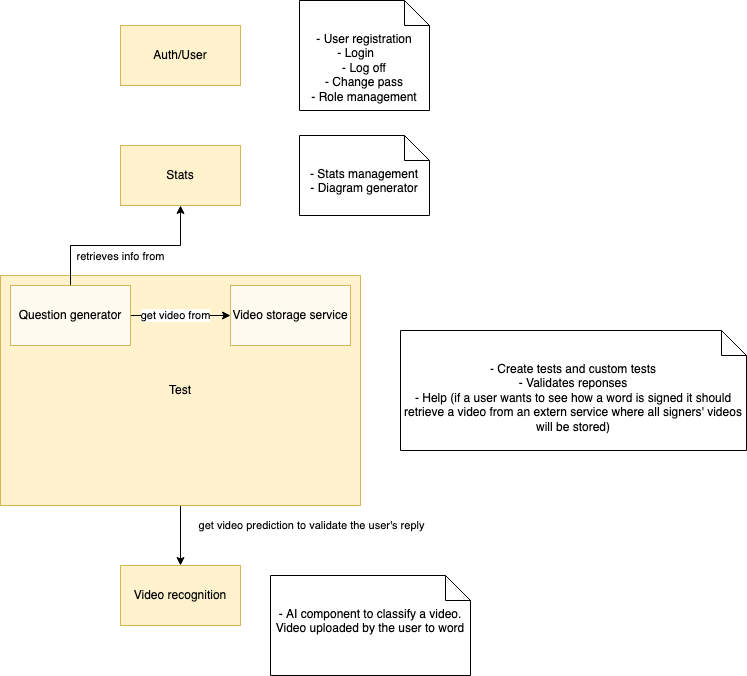
\includegraphics[width=\textwidth]{assets/diagrams/services.png}
    \caption{Towards the app's architecture}
    \label{fig:design_architecture_first}
\end{figure}

Reiterating the last diagram, I got this one, which specifies better the entities. The user communicates with the app, which is formed by the four subsystems. I can have two databases, one for user identification (\textbf{Auth}) and another one for user stats, info about the tests done by them...(\textbf{User stats}). \\

The main difference now is the communication part: the \textit{stats service} does not need to communicate with the \textit{test service}, as the stats can be dynamically created from the info of the database. 

\begin{figure}[H]
    \centering
        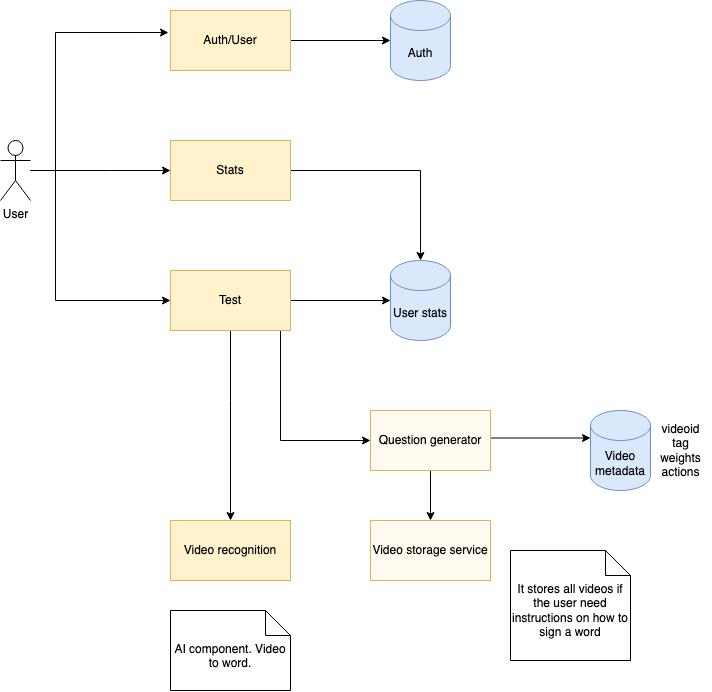
\includegraphics[width=\textwidth]{assets/diagrams/architecture.png}
    \caption{App's architecture}
    \label{fig:design_architecture_last}
\end{figure}

\section{Conceptual design}
As I finally came to understand the better the entities of the application and their relationship, I created a new diagram to simplify all of them. \\

By doing this diagram, I got clearer that the event that changed the stats was the case when a user does a test. Also, I got a new entity: \textit{Question}, which is the base component to form a test. The question comes from the \textit{question generator}, that using the \textit{video storage service} (which can be an extern service) and the \textit{dataset} creates the questions.

\begin{figure}[H]
    \centering
        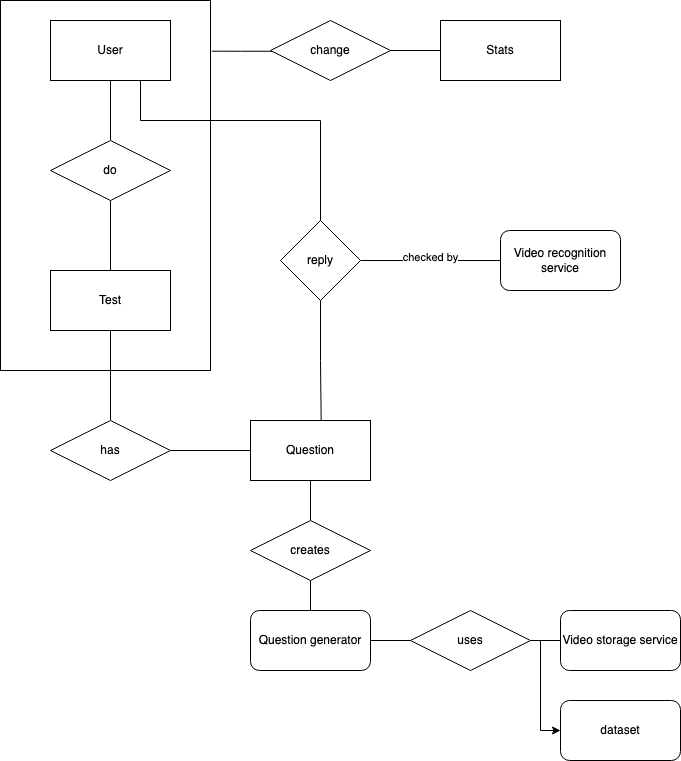
\includegraphics[width=\textwidth]{assets/diagrams/conceptual.png}
    \caption{App's architecture}
    \label{fig:design_conceptual}
\end{figure}

\section{UI design}
\subsection{Low fidelity design}
To validate all the features that the application should have, the navigation, implementation of user stories, design patterns...I created a low-fidelity design. \\

Firstly, I present all the screens created drawing in a tablet. Then, I present the navigation between these screens, so that you can see the flow of the application and how \\
an user should interact with the app itself. \\

I used a mobile as the device as this is the minimum hardware neccessary to use the application and most users nowadays use mobile devices. \\
In order to launch a viable product, I should research the neccessities of these users and study their behaviour. This way, I could know if most of the users \\
wanted to use their pc, tablet instead of mobile devices or they had additional hardware such as external cameras or support devices so that they can use both hands with \\
their mobiles in order to sign correctly. As I don't have the resources and knowledge to do a really useful study of this kind, I selected the minimum device unit and \\
a type of product and tools that could then be migrated to any device (web technology using React could be used in any device and then be migrated to React Native or a PWA reusing most of the components).\\
\subsubsection{Common}
These are the commons components for the whole application. The \textbf{navbar} and the \textbf{bottom bar}. \\

The \textbf{navbar} shows basic information about the current user and allow a quick navigation to secondary info about the app. \\
It could have information about the current page, but this won't be neccessary as I apply the \textit{3-step rule} and there is no much information in this application. \\
What it is important about the navbar, it is that it will allow the navigation to the last page.

The \textbf{bottom bar} allow the user to navigate through the main pages of the application. It won't be visible in subpages to allow the user to concentrate in a task and \\
gain space in the screen. \\
\begin{figure}[H]
    \centering
    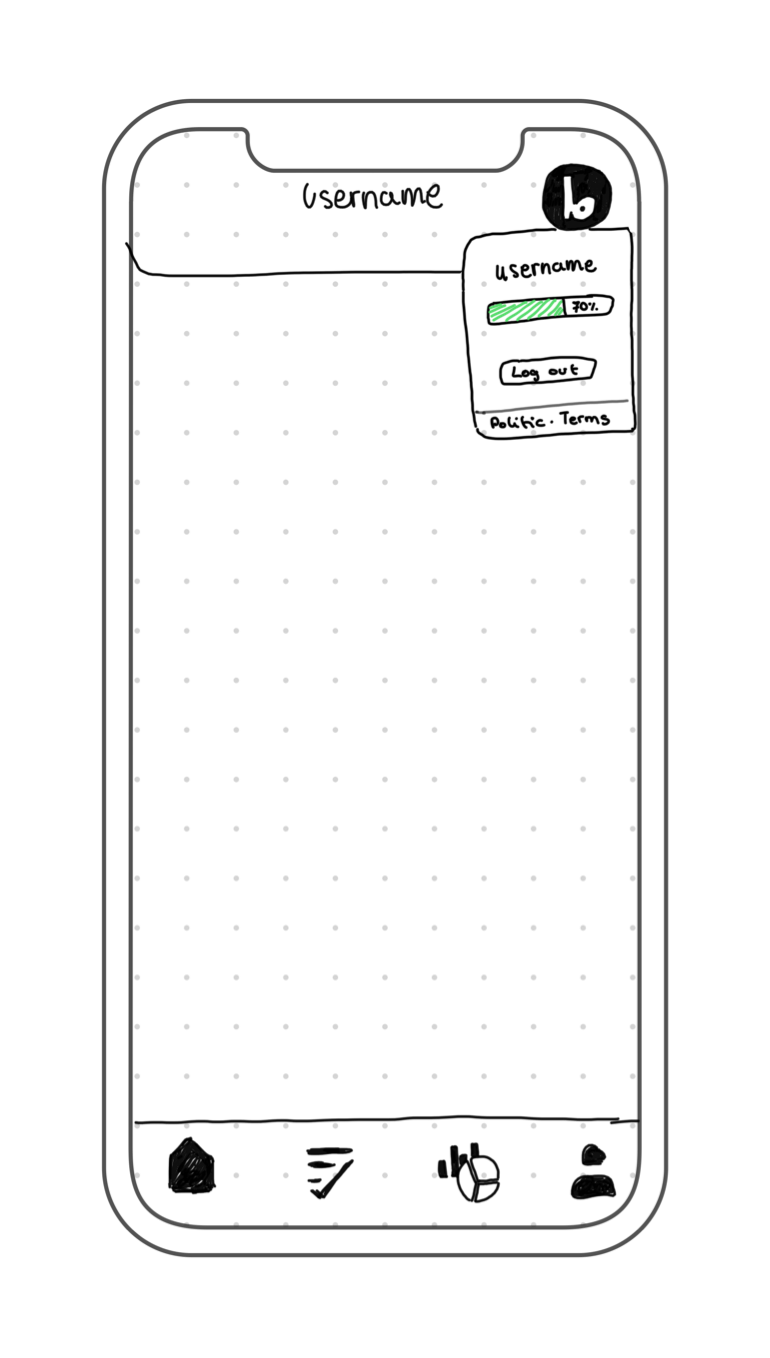
\includegraphics[width=0.24\textwidth]{assets/screens/Button - User.png}
    \caption{Common components}
    \label{fig:design_common}
\end{figure}

\subsubsection{Authorization}
These screens just show the initial pages of the application. In order to be used, being logged in is needed, so the user should be firstly registered and then signed in to start a new session.\\

orify: \textit{RF\_1.1} and \textit{RF\_1.2}. \\
\begin{figure}[H]
    \centering
    \begin{subfigure}[T]{0.49\textwidth}
        \centering
        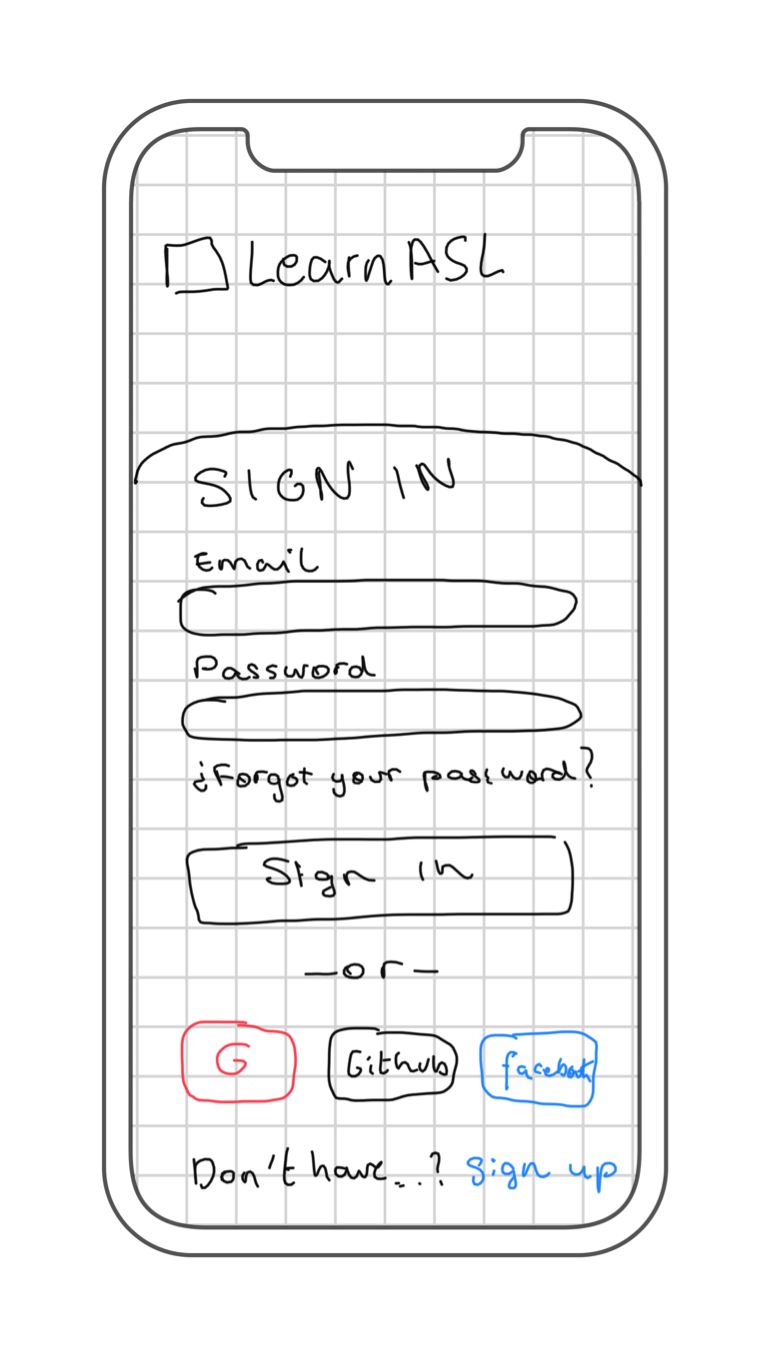
\includegraphics[width=0.48\textwidth]{assets/screens/auth/Login.png}
        \caption{Login screen}
        \label{fig:design_screen_login}
    \end{subfigure}
    \hfill
    \begin{subfigure}[T]{0.49\textwidth}
        \centering
        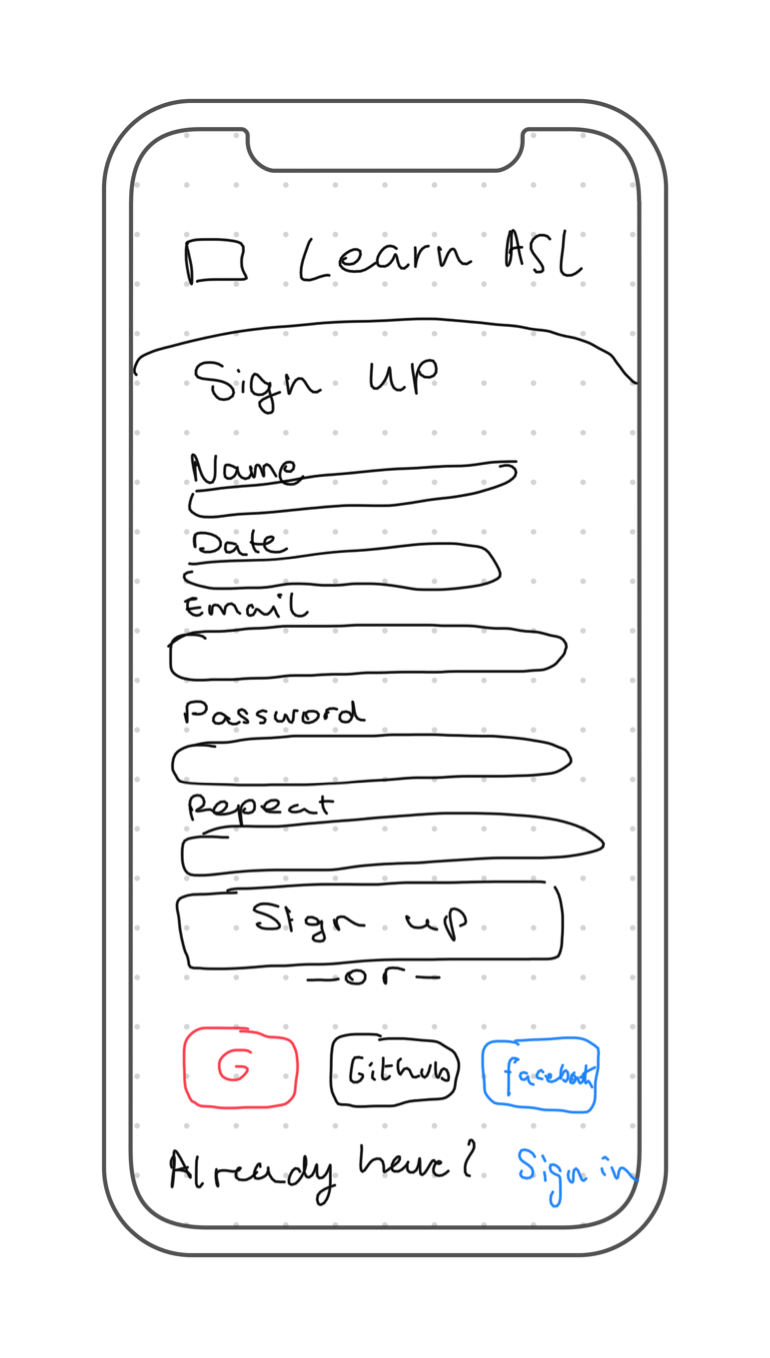
\includegraphics[width=0.48\textwidth]{assets/screens/auth/Register.png}
        \caption{Register screen}
        \label{fig:design_screen_camera_register}
    \end{subfigure}
       \caption{Authorization screens}
       \label{fig:design_screens_auth}
\end{figure}

\subsubsection{Home}
The home screen will show the main information a user want to access. This is the recent quizs taken by the user. \\

In addition, I included an \textbf{ad component}, so that the monetization model of the app could be via ads. This should be taken into account when the app is going to be launched in production and to create a valid business model.\\

It satifies: \textit{RF\_2.3}. \\
\begin{figure}[H]
    \centering
        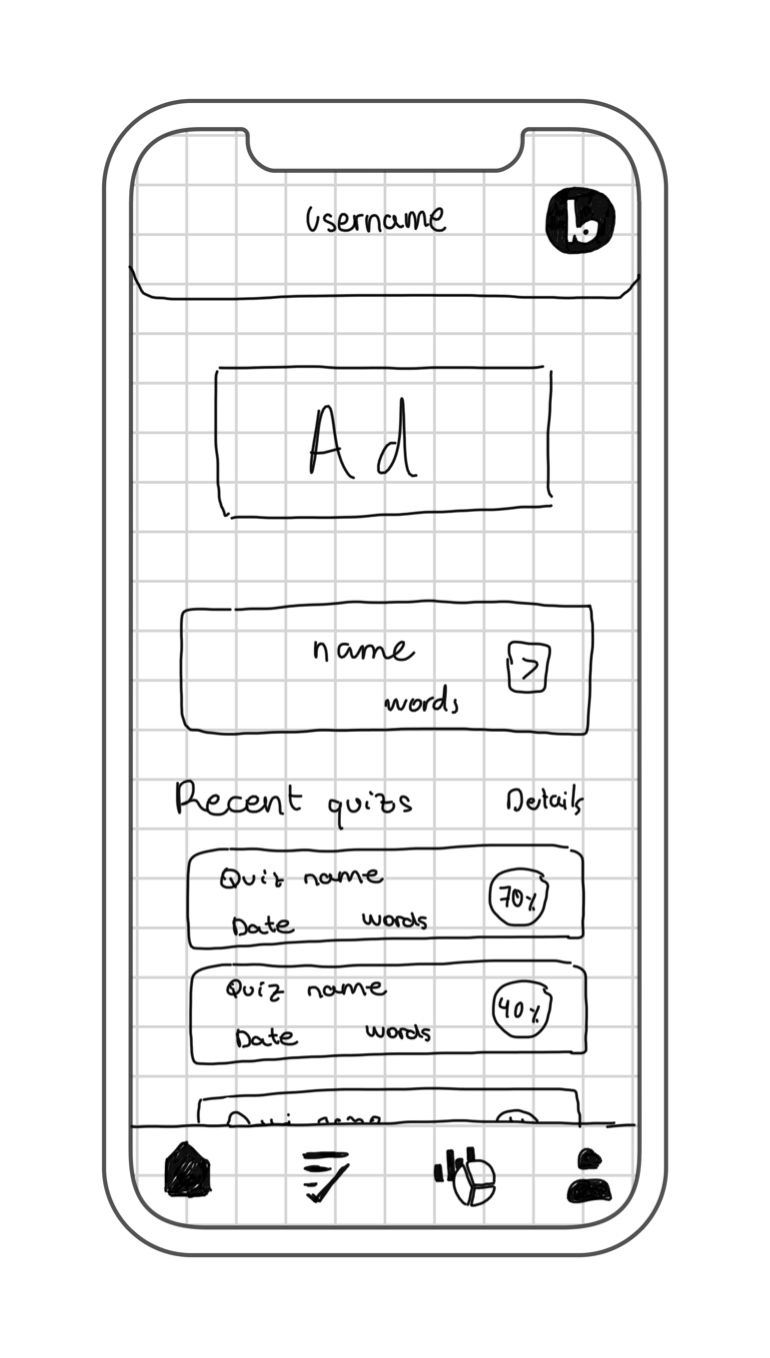
\includegraphics[width=0.24\textwidth]{assets/screens/Home.png}
    \caption{Home screen}
    \label{fig:design_home}
\end{figure}

\subsubsection{Quiz}
These are the common components/screens for the quizs. \\

Firstly, we see a \textbf{result screen}, in which the user can see how they performed doing the current quiz. This could be reusable when the user is reviewing an already done quiz. \\
As the main objective of an user in the application is to do quizes, it has a button to easily access this feature. \\
A share button is included so that the application can gain visibility via users. The main objective of this is not fomenting competitivity, but gaining visibility in social network platforms. \\

Secondly, we see a \textbf{selecting difficulty screen}. The user will be able to customize a quiz, selecting the \textbf{difficulty} and the \textbf{number of questions} of a test. \\

Finally, we see a \textbf{selecting quiz's type screen}. The user will be able to select the \textbf{test type} before starting a new one. \\
\begin{figure}[H]
    \centering
    \begin{subfigure}[T]{0.32\textwidth}
        \centering
        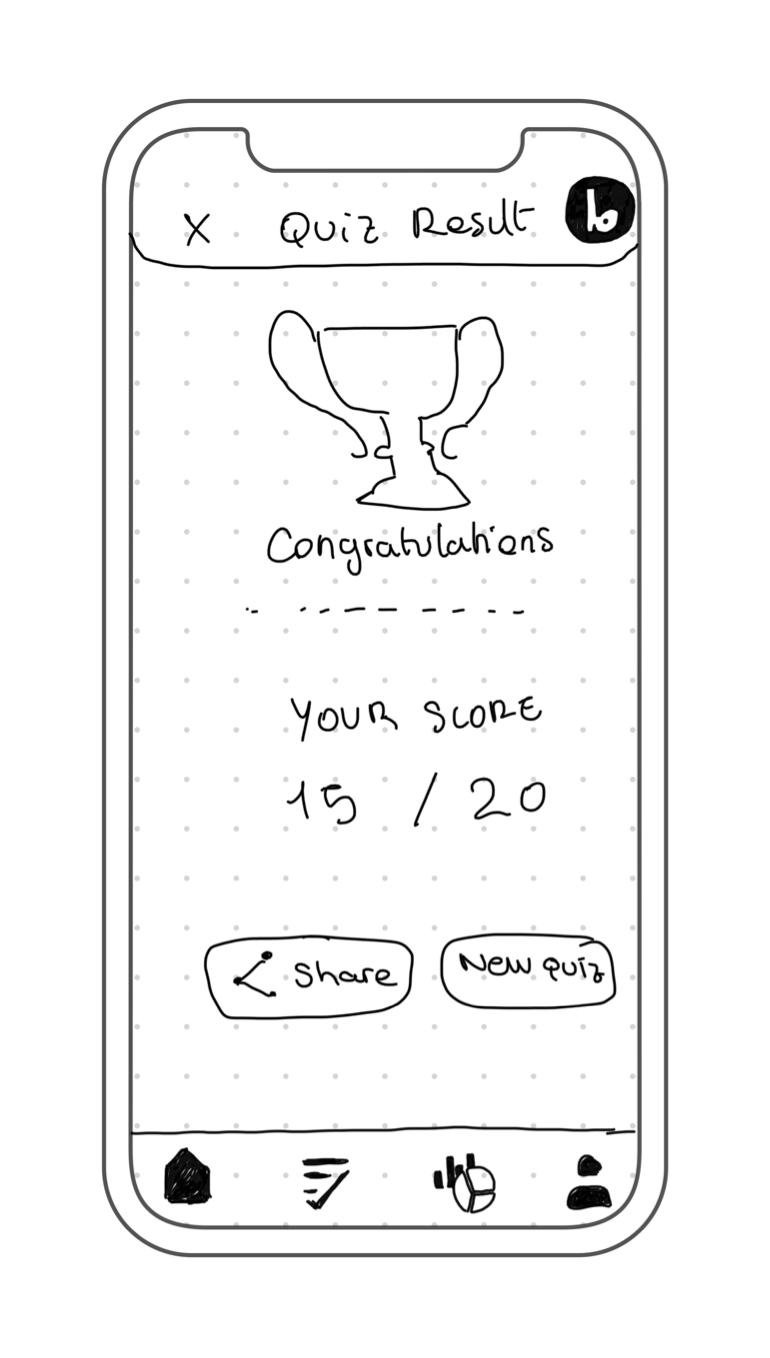
\includegraphics[width=0.72\textwidth]{assets/screens/quiz/common/Quiz - Result.png}
        \caption{Result of a test}
        \label{fig:design_screen_result}
    \end{subfigure}
    \hfill
    \begin{subfigure}[T]{0.33\textwidth}
        \centering
        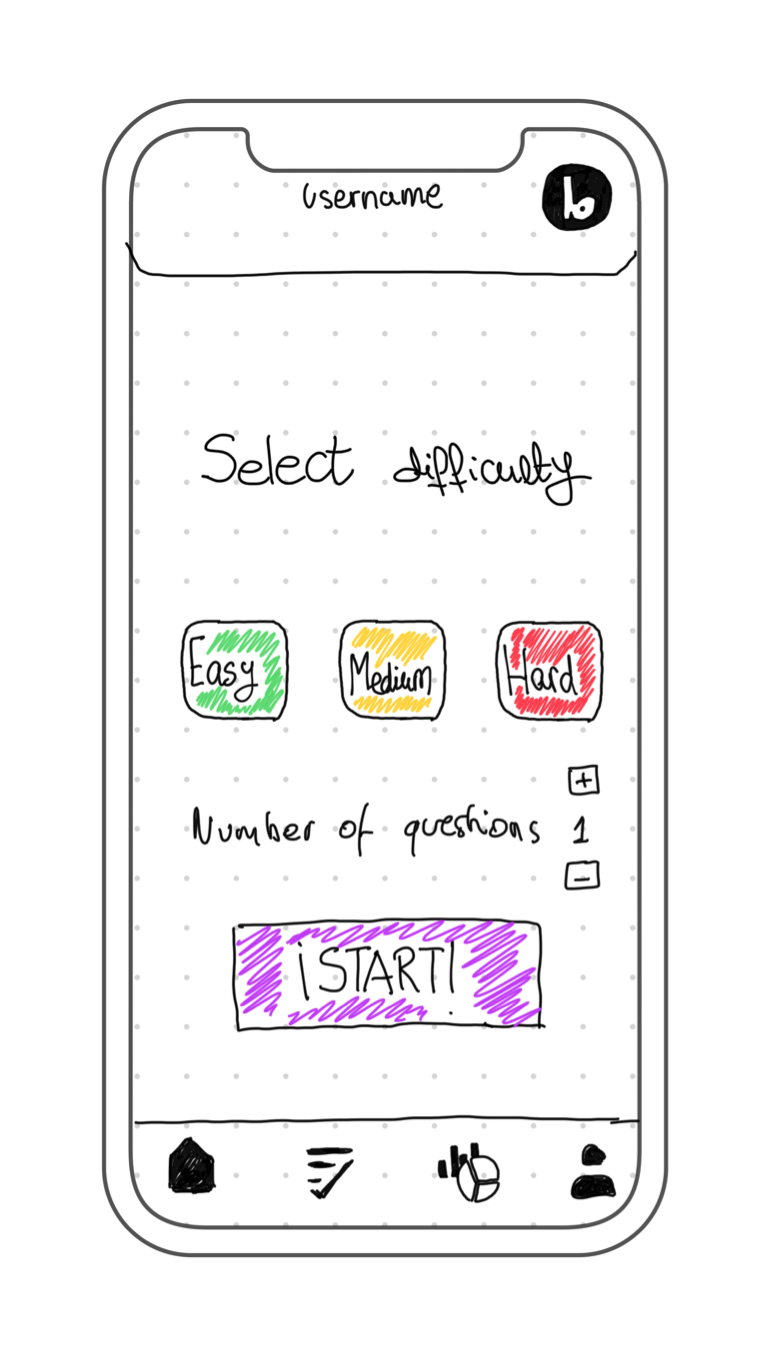
\includegraphics[width=0.72\textwidth]{assets/screens/quiz/common/Select difficulty.png}
        \caption{Select difficulty of a test}
        \label{fig:design_screen_select_dif}
    \end{subfigure}
    \hfill
    \begin{subfigure}[T]{0.33\textwidth}
        \centering
        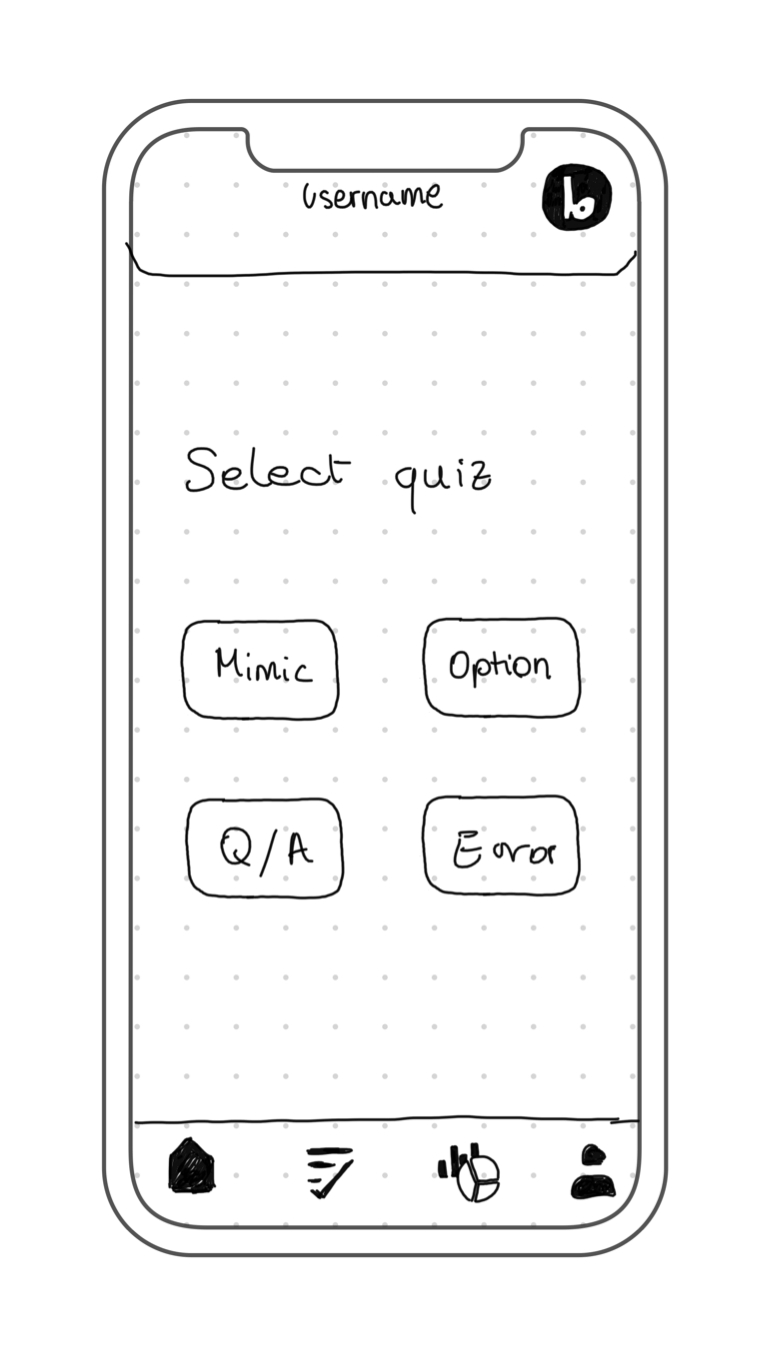
\includegraphics[width=0.72\textwidth]{assets/screens/quiz/common/Select quiz.png}
        \caption{Select type of test}
        \label{fig:design_screen_select_quiz}
    \end{subfigure}
       \caption{Common screens for all tests}
       \label{fig:design_test_common}
\end{figure}
Here I am presenting the quizes themselves. What it is important to notice is that the user can \textbf{skip} a question, see how many questions the current quiz has, the test type and a feedback for the question result, as well as the number of the current question. \\

\begin{itemize}
    \item \textbf{Mimic:} the question is composed by the word to sign and a help video. The user should sign themselves signing that word and can watch the help video to imitate it.
    \item \textbf{Option video to word:} the question is composed by a video representing a sign and 4 options (words). The user should select the word matching the video.
    \item \textbf{Option word to video:} the question is composed by a word and 4 videos representing signs. The user should select the video that signs correctly the asked word.
    \item \textbf{QA:} the question is composed by just the word to sign. The user should sign the word.
\end{itemize}
\begin{figure}[H]
    \centering
    \begin{subfigure}[T]{0.24\textwidth}
        \centering
        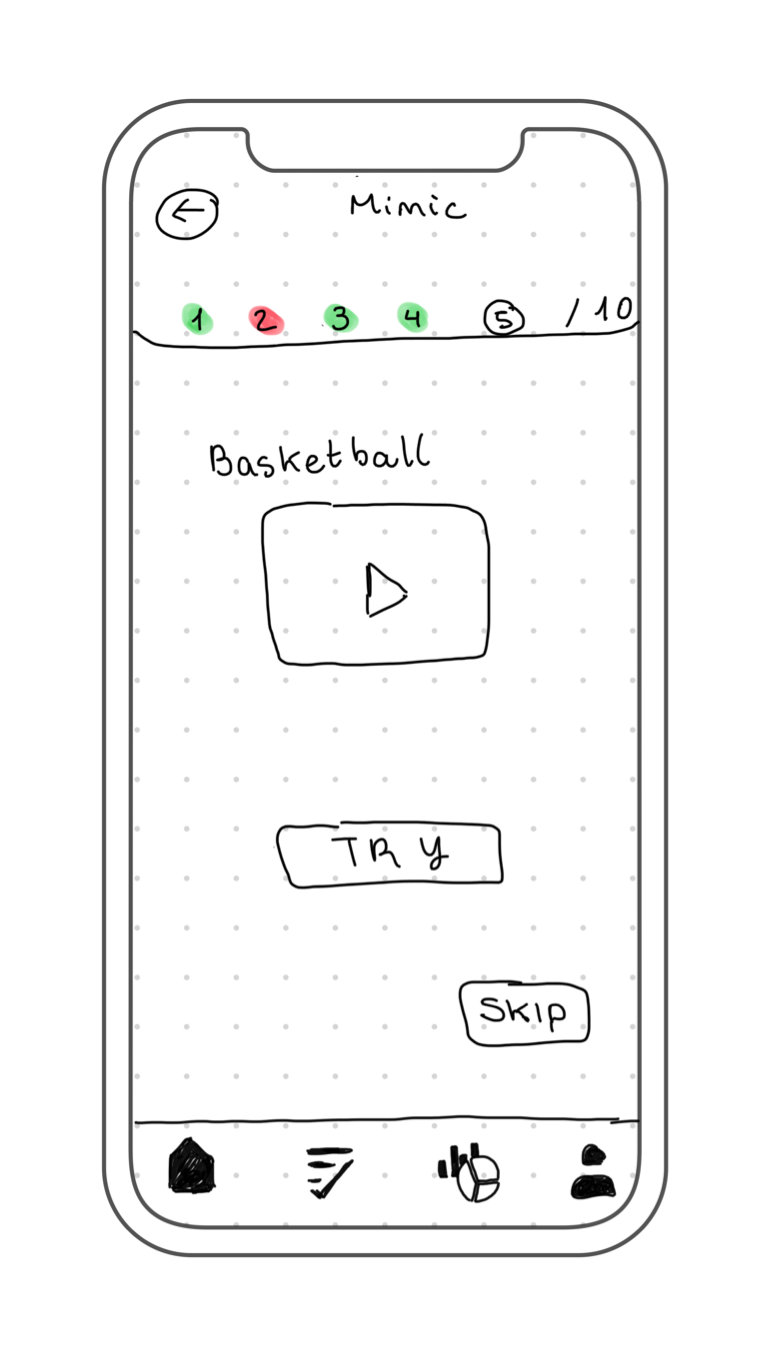
\includegraphics[width=\textwidth]{assets/screens/quiz/Quiz - Mimic.png}
        \caption{Mimic}
        \label{fig:design_screen_mimic}
    \end{subfigure}
    \hfill
    \begin{subfigure}[T]{0.24\textwidth}
        \centering
        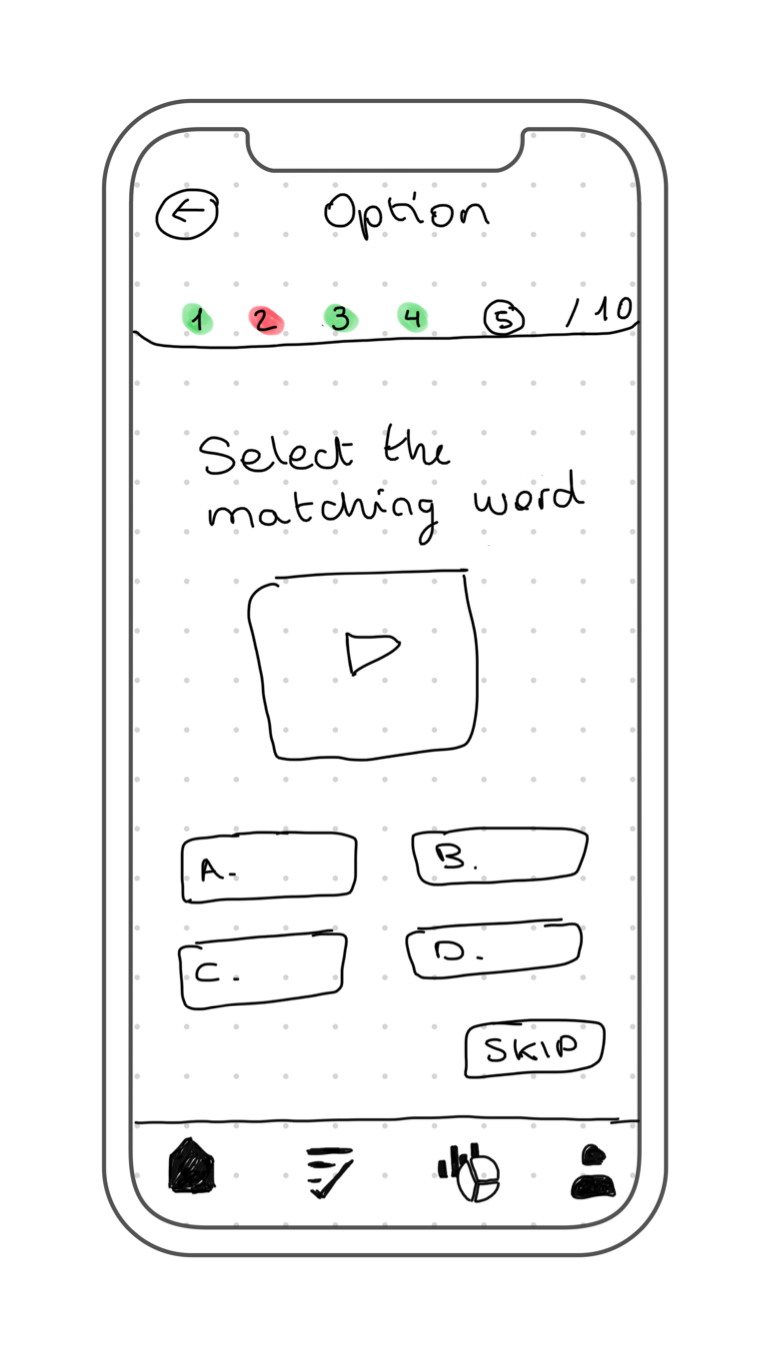
\includegraphics[width=\textwidth]{assets/screens/quiz/Quiz - Option 1.png}
        \caption{Option video to word}
        \label{fig:design_screen_mimic}
    \end{subfigure}
    \hfill
    \begin{subfigure}[T]{0.24\textwidth}
        \centering
        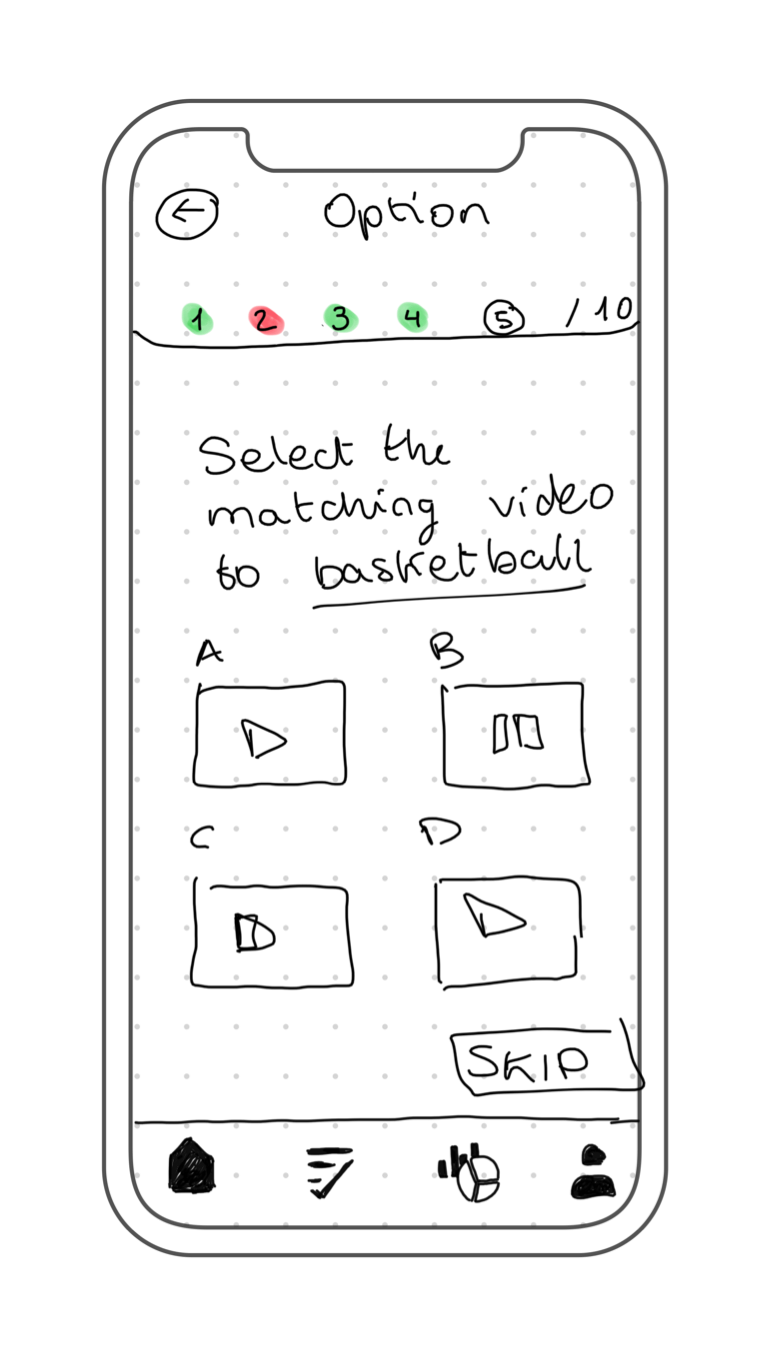
\includegraphics[width=\textwidth]{assets/screens/quiz/Quiz - Option 2.png}
        \caption{Option word to video}
        \label{fig:design_screen_mimic}
    \end{subfigure}
    \begin{subfigure}[T]{0.24\textwidth}
        \centering
        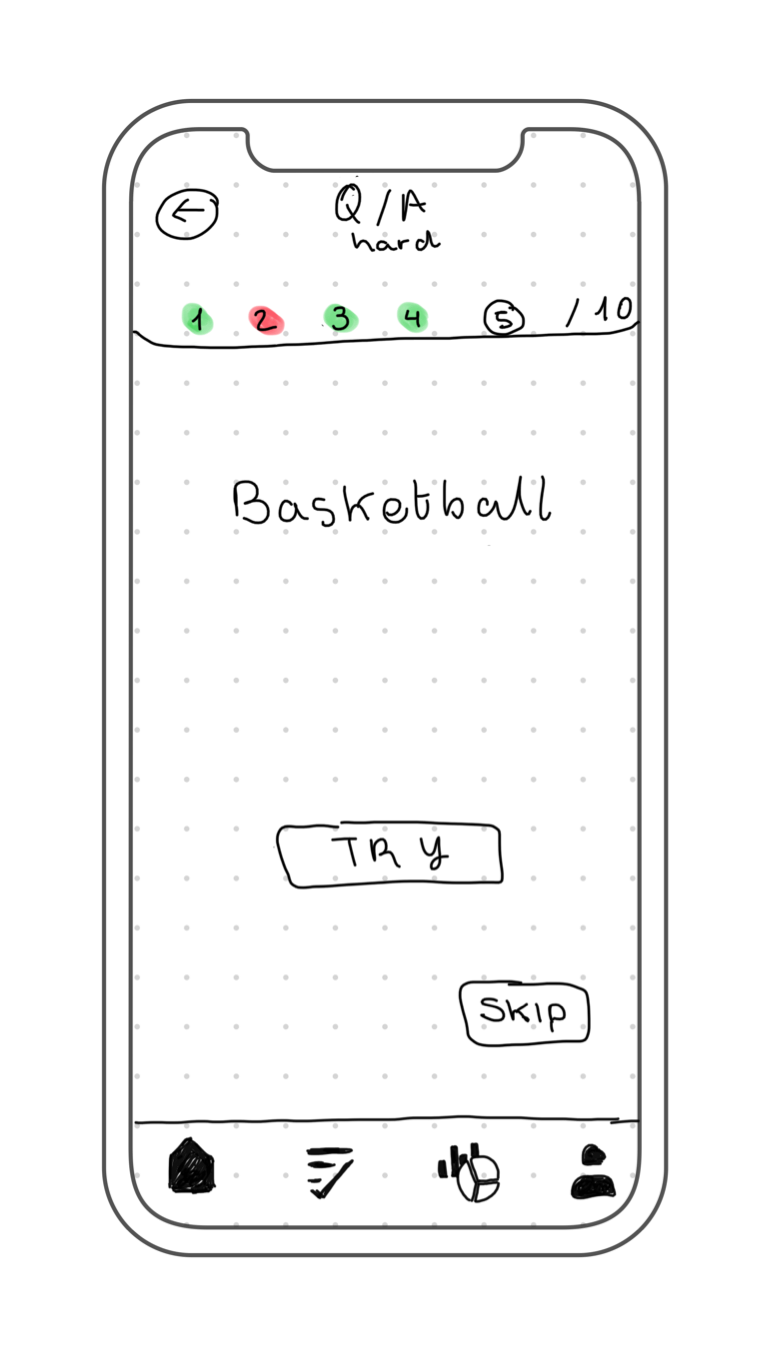
\includegraphics[width=\textwidth]{assets/screens/quiz/Quiz - Q_A.png}
        \caption{QA}
        \label{fig:design_screen_mimic}
    \end{subfigure}
       \caption{Tests' screens}
       \label{fig:design_test_screen}
\end{figure}

These screens represent how a user could reply to a question if they are asked to send a video. They could select a video from the gallery or record them signing the word, and send the video to the application or record it again. \\
\begin{figure}[H]
    \centering
    \begin{subfigure}[T]{0.49\textwidth}
        \centering
        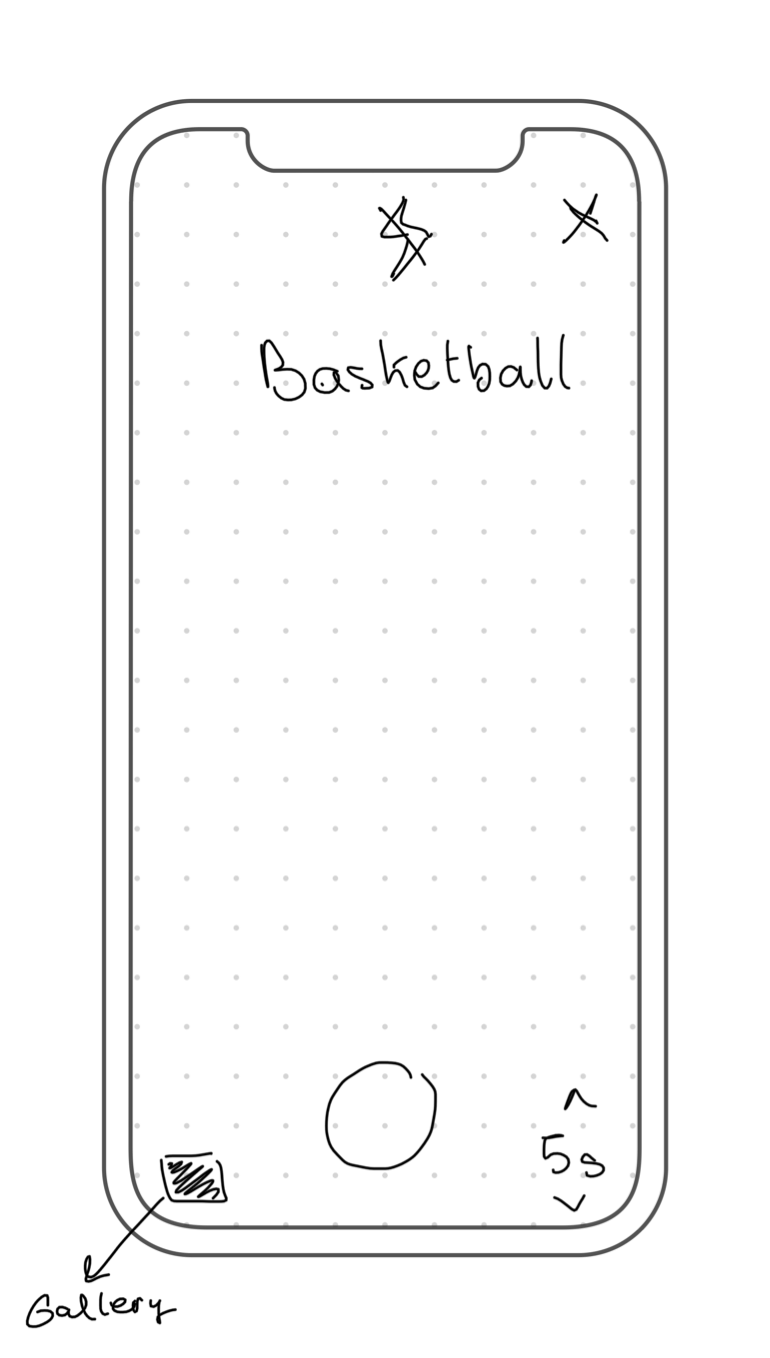
\includegraphics[width=0.48\textwidth]{assets/screens/quiz/quiz-camera/Quiz - Camera.png}
        \caption{Camera}
        \label{fig:design_screen_camera}
    \end{subfigure}
    \hfill
    \begin{subfigure}[T]{0.49\textwidth}
        \centering
        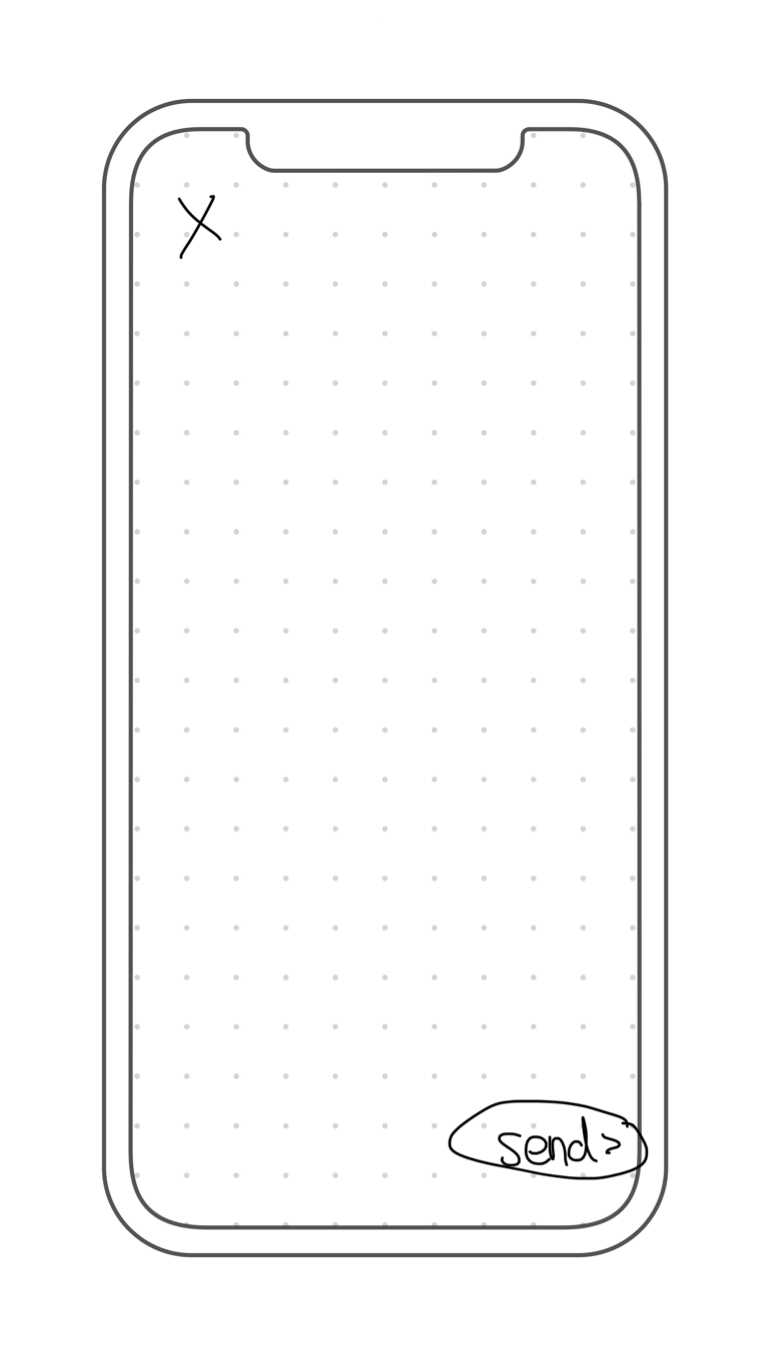
\includegraphics[width=0.48\textwidth]{assets/screens/quiz/quiz-camera/Quiz - Camera send.png}
        \caption{Send photo}
        \label{fig:design_screen_camera_send}
    \end{subfigure}
       \caption{Reply to test using the camera}
       \label{fig:design_camera}
\end{figure}

\subsubsection{Stats}
In order to show the stats to the user, a stat screen is added. \\

The first screen represent the most basic information: the \textbf{percent of learnt words} and the \textbf{use of the app} (in the calendar an user can see the days they have used the application starting a new quiz). They also can consult the maximum number of days they have used the application in a row and the current streak. \\

The second screen shows more information about the app to the user: \textbf{time spent} in the app and \textbf{new words learnt}, as well as the \textbf{success rate}. The users can filter the stats by date (and/or) by difficulty. \\

The third screen show another way of representing the stats, in a more detailed way using graphs. \\

orify: \textit{RF\_3.1} and \textit{RF\_3.2}. \\
\begin{figure}[H]
    \centering
    \begin{subfigure}[T]{0.32\textwidth}
        \centering
        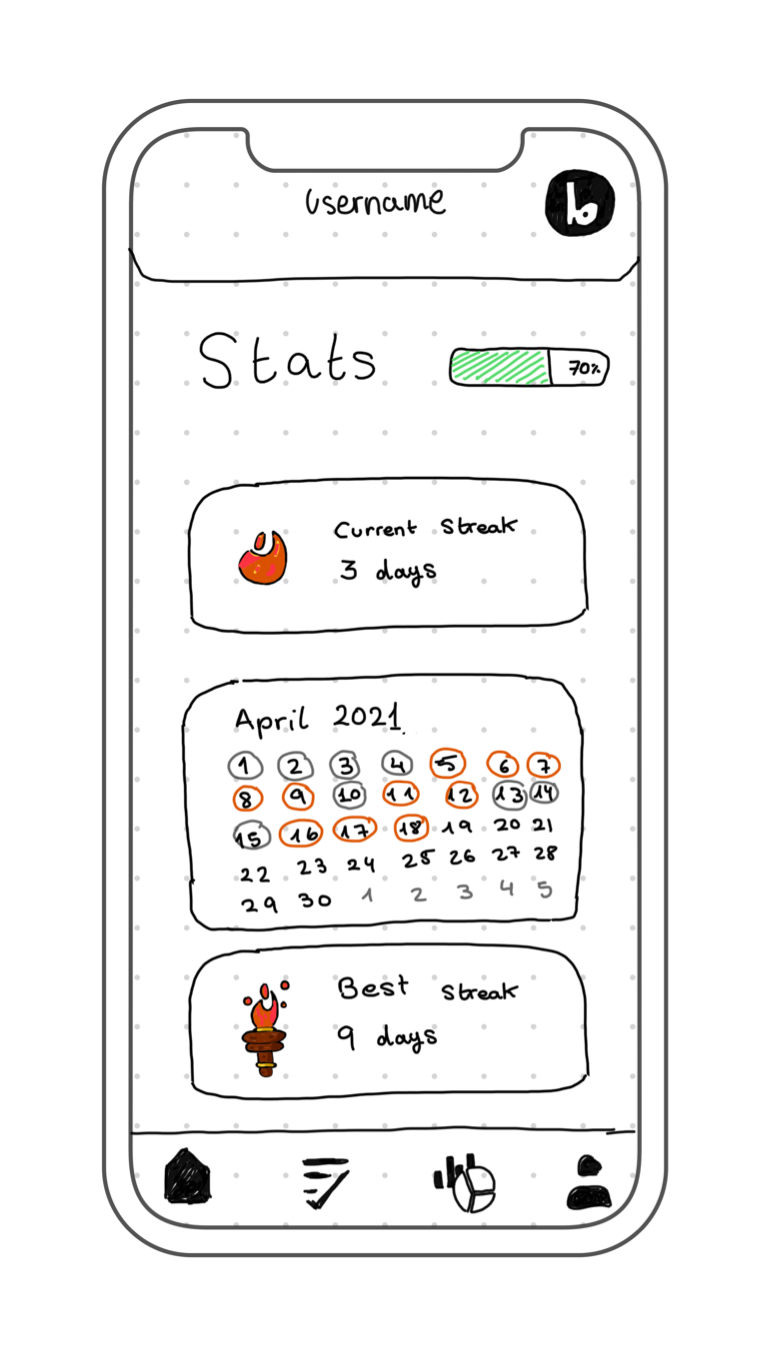
\includegraphics[width=0.72\textwidth]{assets/screens/stats/Stats - 1.png}
        \caption{Stats: page 1}
        \label{fig:design_screen_stats_1}
    \end{subfigure}
    \hfill
    \begin{subfigure}[T]{0.32\textwidth}
        \centering
        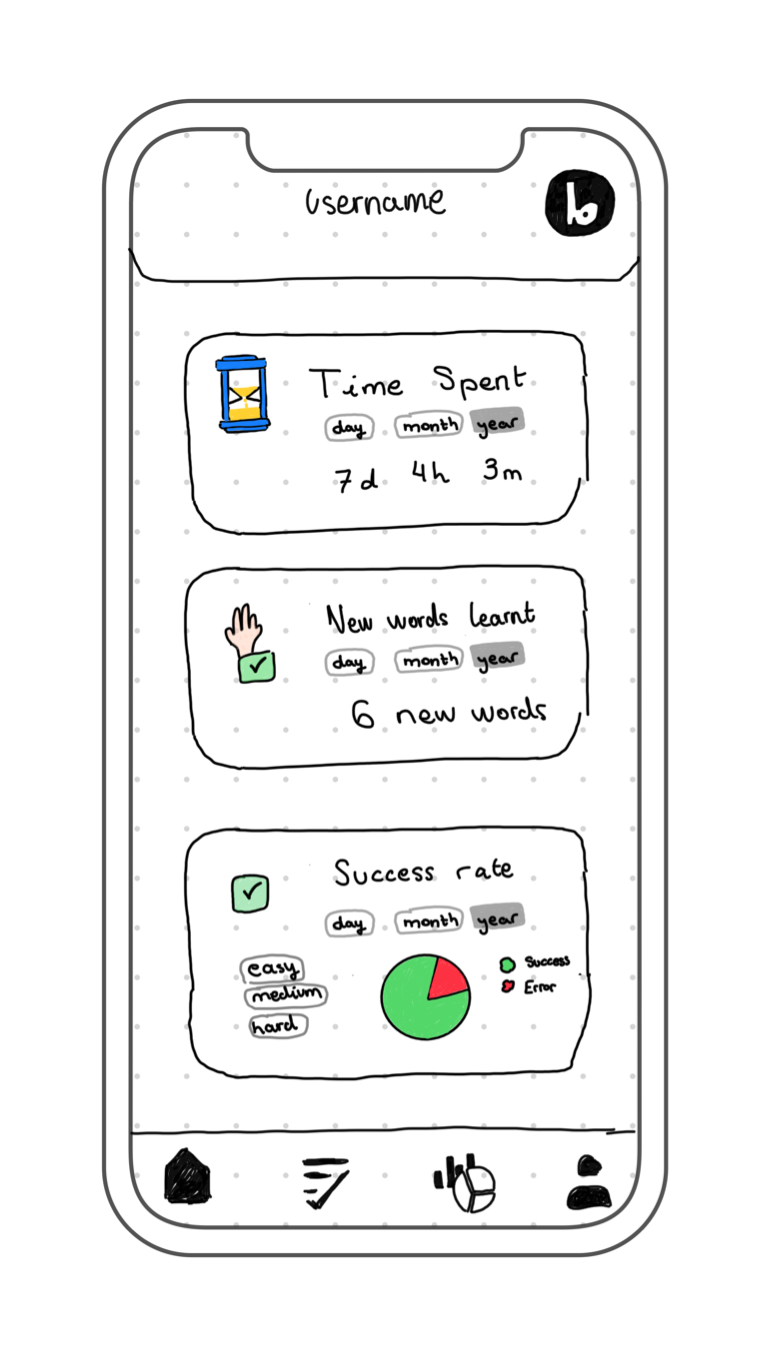
\includegraphics[width=0.72\textwidth]{assets/screens/stats/Stats - 2.png}
        \caption{Stats: page 2}
        \label{fig:design_screen_stats_2}
    \end{subfigure}
    \hfill
    \begin{subfigure}[T]{0.32\textwidth}
        \centering
        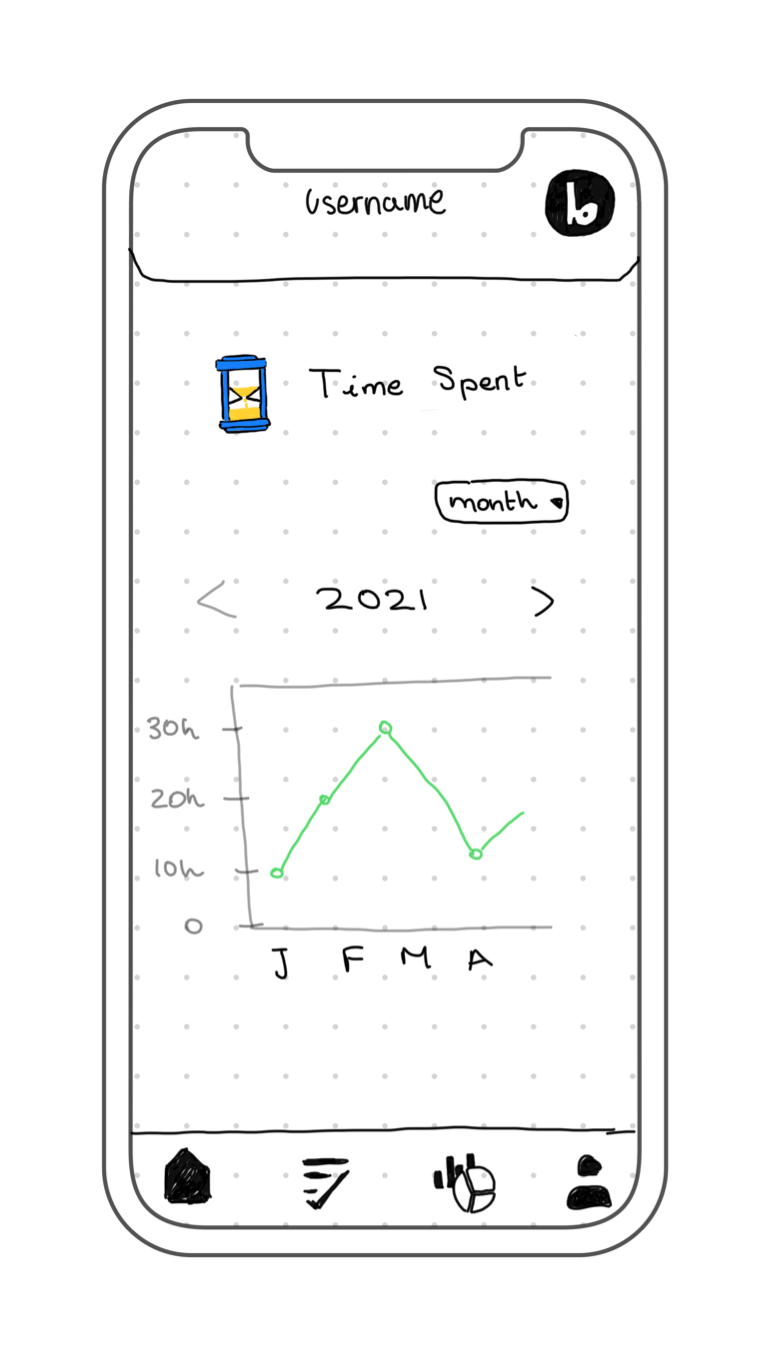
\includegraphics[width=0.72\textwidth]{assets/screens/stats/Stats - 3.png}
        \caption{Stats' detail}
        \label{fig:design_screen_stats_3}
    \end{subfigure}
       \caption{Stats' screens}
       \label{fig:design_screen_stats}
\end{figure}

\subsubsection{User}
This screen allow the user to customize the application and change personal information. \\
\begin{figure}[H]
    \centering
        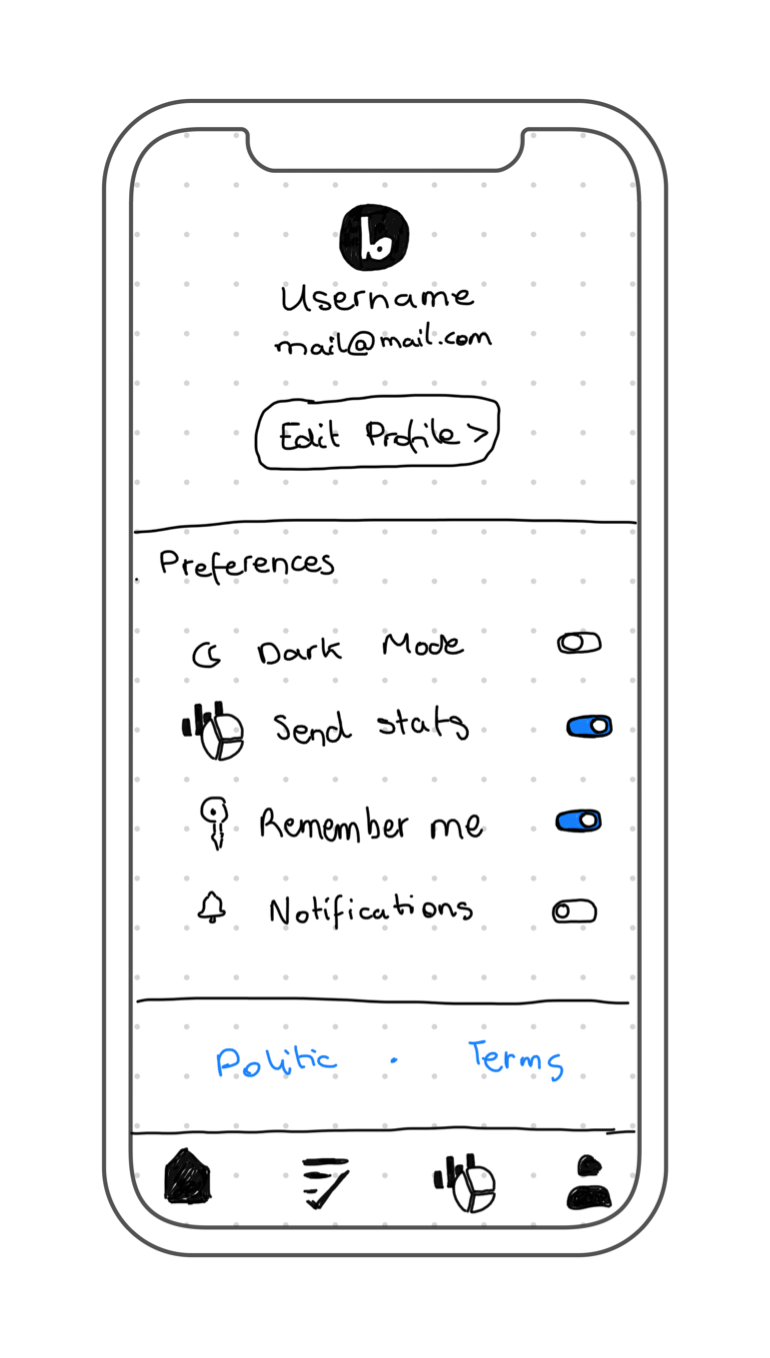
\includegraphics[width=0.24\textwidth]{assets/screens/User.png}
    \caption{User screen}
    \label{fig:design_user}
\end{figure}

\subsubsection{Navigation}
In this figure we can see how a user would interact with every screen and the navigation between all of them. \\

Firstly, there is a first layer that the user has to pass, which is the auth layer. In order to use the rest of the application (private routes), the user \\
should sign in the application. \\

Secondly, there is a row containing the main screens of the application. Using the \textbf{bottom bar} the user is able to move from one to another. \\

Finally, we see all the rest of the subpages of the application, that contains more detailed information or actions. Among them we can see more in-detail stats \\
or doing/reviewing quizes.
If we take a look into the quiz ramification, we see a use case: create a test and do it. The user first customize the quiz, selecting the difficulty, number of questions and type of quiz. Then the user reply to the questions of the quiz itself and then the user is able to see the quiz result.\\

\begin{figure}[H]
    \centering
        \includegraphics[width=\textwidth]{assets/lofi.png}
    \caption{Low-fidelity design}
    \label{fig:design_lofi}
\end{figure}



	% Desarrollo bajo sprints: 
	% 	1. Permitir registros y login de usuarios
	% 	2. Desarrollo del sistema de incidencias
	% 	3. Desarrollo del sistema de denuncias administrativas y accidentes
	% 	4. Desarrollo del sistema de croquis
	%   5. Instalación de la aplicación de manera automática
	\chapter{Implementation}

La implementación del software se ha dividido en hitos. Estos, han sido definidos en Github
y cada uno de ellos contiene un grupo de \textit{issues} que se corresponden con las distintas
mejoras que se han ido incorporando al software a lo largo de su desarrollo.\\



	\chapter{Testing}

\section{Definition of all tests}

\section{Unit tests}
\subsection{Implementation}
\subsection{Execution}

\section{Integration tests}
\subsection{Implementation}
\subsection{Execution}

\section{Continious integration}
	% Presupuesto

	% Conclusiones
	\chapter{Conclusions and future work}

This project has served me as my presentation letter to the job market and has given me the opportunity to learn industry-standard 
technologies and development methodologies used in companies nowadays. This is due to my attitude towards the project itself, as I 
did not want to simply meet the requirements of the project, but to do a job that can really serve people (a social purpose and a 
usable product) and that allows me to learn cutting-edge technologies and choose the branch of computer science that I find the most 
attractive (full-stack development or data science).
In addition to fulfilling the technical requirements to deliver this work, I have fulfilled my own personal and professional goals. \\

The first stages of the development process of this project were useful for me to learn more about deep learning, since in my study-branch 
(Software Development) we do not study this area of knowledge. Also, it helped me to learn how to read scientific articles and develop my 
project ideation, as the proposal for the development of the project was suggested by me.
The later stages helped me to learn which technologies were used in the industry and to focus on those that were convenient for this project. 

After a whole development process in which I have learned to use version control, divide a project into milestones and user stories, 
develop prototypes, create an REST API, make use of an API from a frontend, create a microservice that uses a machine learning model and 
perform unit and integration tests, I think I have grown as a developer. I have applied many concepts learned in my degree and I have 
learned to use them in a real environment. Also, personally, I have more confidence to be able to transform an idea into a software product, 
I feel better having developed a product that can help people at risk of exclusion and it has allowed me to find my first job. \\

Although the overall balance is positive, I am critical and there are some decisions I should have made. 
One of them is to avoid using beta versions of products. Although I used it to learn and because I found it attractive, it was an unnecessary 
cost for me to change every time the version was updated.
Another decision I would rethink would be to use a test-driven methodology, such as TDD (Test Driven Development). 
This is because in the end I implemented unit tests, but it would have saved me manual debugging time.
Also, I was lucky to have enough time to invest in the project. I would have chosen a topic that covered fewer technologies and topics, 
because, if I had been in another situation, it would have been unfeasible to complete it. \\

From this work, the scientific community can gain much value. 
The first contribution of this work for future works is that it can make use of the \textbf{literature review} \ref{LiteratureReview} that I carried out, where I analyze 
the state of art and provide insights about the existing approaches, models and datasets.
Finally, \textbf{ideas} are offered for new applications to help the deaf-and-dumb community (integration of such a model at a conversational 
level in video call applications such as Jitsi \cite{Jitsi} so that non-signing users and signing users can interact in the same meeting).

	% Trabajos futuros

	\backmatter
	\begingroup
		\setlength\parindent{0pt}
		\chapter{Glosario de términos}

\textbf{Backend}: part of a web application that the user does not see. It is responsible of replying to every user request and doing an action on every one. Among these actions it could store data, send stored data, communicate with other service...
\bigskip

\textbf{Frontend}: part of a web application that the user really see. It is the layer between the user and the backend.
\bigskip

\textbf{HTTP}: \textit{HyperText Transfer Protocol}, it enables the communication between client and server. 
\bigskip

\textbf{HTTPS}: \textit{HTTP Secure}. Encrypted version of HTTP.
\bigskip

\textbf{URL}: \textit{Uniform Resource Locator}, location of an object on a computer network.
\bigskip

\textbf{Header}: field of an HTTP request or response to send additional information.
\bigskip

\textbf{Body}: payload of an HTTP request or response.
\bigskip

\textbf{Metadata}: information about the thing that the client retrieves from an HTTP response.
\bigskip

\textbf{Form-data}: interface to construct a set of key/value pair to send information in an HTTP request.
\bigskip

\textbf{Params}: name-value pairs to request particular resources from a web server using HTTP.
\bigskip

\textbf{Map}: data structure that stores key-value pairs. There cannot be duplicate keys. The keys are used to access the element and its data (value).
\bigskip

\textbf{Lifetime}: also called \textit{life cycle}. Time between an object's creation and its destruction.
\bigskip

\textbf{Authorization}: process of verifying what specific resources an user has acess to.
\bigskip

\textbf{Authentication}: process of verifying who someone is.
\bigskip

\textbf{CORS}: \textit{Cross-Origin Resource Sharing}, is an HTTP-header based mechanism that allows a server to indicate any origin.
\bigskip

\textbf{State management}: in a Web UI Framework, it enables the application to remember a user interface state and apply it. Therefore, the UI of the application would be different according of the current state of the application.
\bigskip

\textbf{UI}: \textit{User Interface}, is the point of human-computer interaction and communication in a device.
\bigskip

\textbf{Component}: a part or element of a larger whole. In Web development, it refers to a part of the webpage. It can be reusable and it has its own responsability and state.
\bigskip

\textbf{Redux}: design pattern to manage the state of an application. 
\bigskip

\textbf{REST}: \textit{REpresentational State Transfer} is a software architectural style that was created to guide the design and development of the architecture for the WWW. It realies on a stateless, client-server protocol.
\bigskip

\textbf{API}: \textit{Application Programming Interface} is a software intermediary that allows two applications to communicate with each other.
\bigskip

\textbf{Design pattern}: in software design, it is a typical solution to resolve common problems. It is like a blueprint that you can customize to solve a particular problem in your application.
\bigskip

\textbf{Software Architecture}: organization of a system. It includes all components, how they interact with each other, the evolution...
\bigskip

\textbf{Software}: it is a set of instructions, data or programs used to operate computers.
\bigskip

\textbf{Clean Architecture}: is a software design philosophy that separates the elements of a design into ring levels.
\bigskip

\textbf{Scrum}: it is a framework used for project management that emphasizes teamwork, accountability and iterative progress toward a well-defined goal.
\bigskip

\textbf{Sprint}: it is a short, time-boxed period when a scrum team works to complete a set amount of work.
\bigskip

\textbf{State of art}: refers to the highest level of development that has been achieved to date in a design, process, material or technique and is a key point in any industrial engineering project.
\bigskip

\textbf{Product backlog}: it is a list of the new features, changes to existing features, bug fixes, infrastructure changes or other activities that a team may deliver in order to achieve a specific outcome. 
\bigskip

\textbf{Bug}: it is an error, flaw or fault in computer software that causes it to produce an incorrect or unexpected result, or to behave in unintended ways.
\bigskip

\textbf{Milestone}: it is a marker of a stage in a project. 
\bigskip

\textbf{MVP}: \textit{Minimum Viable Product}, is a product with enough features to attract early-adopter customers and validate the product idea. It is the first product to develop in order to get early feedback from real users.
\bigskip

\textbf{Kanban}: it is a method to manage work. A kanban table could divide the tasks in \textit{To do}, \textit{Doing}, \textit{To review}, \textit{Reviewing}, \textit{Done}. 
\bigskip

\textbf{User story}: it is a tool in agile development used to capture a description of a task from an user's perspective.
\bigskip

\textbf{Agile}: method of project management.
\bigskip

\textbf{Unit test}: software development process in which the smallest components and parts of the application (units) are tested.
\bigskip

\textbf{Integration test}: software development process in which the units are tested combined.
\bigskip

\textbf{Framework}: it is a standard, abstraction or template that gives to developers all the tool required to achieve a software product.
\bigskip

\textbf{Continuous integration}: software development practice in which developers merge their code changes into a repository, after automated builds and tests.
\bigskip

\textbf{Repository}: it is a central place to store, aggregate data and change data in a mainteined and organized way.
\bigskip

\textbf{Deep Learning}: type of machine learning and artificial intelligence that imitates the way humans gain certain types of knowledge. It includes statistics and predictive modelling.
\bigskip

\textbf{Model}: the deep learning element that performs classification or predictive tasks. 
\bigskip

\textbf{Dataset}: collection of data.
\bigskip

\textbf{Open source}: software that people can modify, see, share and use because its design and development is publicly accesible.
\bigskip

\textbf{Convolution}: mathematical operation on two functions that produces a third function that expresses how the shape of one is modified by the other.
\bigskip

\textbf{Layer}: it is a structure in a deep learning model that take information and pass information to the next layer.
\bigskip
	\endgroup


	
	\newpage
	\bibliography{bibliografia}
	\bibliographystyle{plain}
	
\end{document}

